\documentclass[12pt,a4paper]{article}
\usepackage[a4paper, margin=0.8in, headheight=14pt]{geometry}
\usepackage{fontspec}
\usepackage{unicode-math}
\setmainfont{TeX Gyre Pagella}
\setmonofont[Scale=0.88]{TeX Gyre Cursor}
\setmathfont{Latin Modern Math}
\usepackage{xcolor}
\usepackage{colortbl}
\usepackage{titlesec}
\usepackage{enumitem}
\usepackage{tabularx}
\usepackage{booktabs}
\usepackage{array}
\usepackage{amsmath}
\usepackage{tikz}
\usetikzlibrary{shapes.geometric, arrows.meta, positioning, calc, fit, decorations.pathreplacing, decorations.pathmorphing, patterns}
\usepackage[american]{circuitikz}
\usepackage{tcolorbox}
\tcbuselibrary{skins, breakable}
\usepackage{hyperref}
\usepackage{fancyhdr}
\usepackage{graphicx}
\usepackage{microtype}
\hyphenpenalty=10000
\exhyphenpenalty=10000
\sloppy
\usepackage{caption}
\usepackage{setspace}
\usepackage{multirow}
\usepackage{tocloft}
\newcommand{\Q}[1]{\textbf{#1}\par\noindent\ignorespaces}
\definecolor{myred}{RGB}{196,30,58}
\definecolor{mydark}{RGB}{30,30,50}
\definecolor{mygreen}{RGB}{14,120,80}
\definecolor{myteal}{RGB}{0,130,140}
\definecolor{myamber}{RGB}{180,100,0}
\definecolor{mypurple}{RGB}{100,30,160}
\definecolor{mygray}{RGB}{246,247,249}
\definecolor{mgframe}{RGB}{180,185,200}
\definecolor{watermark}{RGB}{145,150,170}
\definecolor{hdrred}{RGB}{250,232,235}
\definecolor{hdrgreen}{RGB}{220,244,233}
\definecolor{hdrteal}{RGB}{220,242,244}
\definecolor{hdramber}{RGB}{253,242,215}
\definecolor{hdrpurple}{RGB}{238,228,255}
\definecolor{hdrgray}{RGB}{238,240,245}
\definecolor{rowalt}{RGB}{250,251,253}

\titleformat{\section}{\large\bfseries\color{myred}}{\thesection.}{0.5em}{}[\vspace{1pt}{\color{myred}\rule{\linewidth}{0.8pt}}]
\titleformat{\subsection}{\normalsize\bfseries\color{myteal}}{\thesubsection}{0.5em}{}
\titlespacing*{\section}{0pt}{18pt}{7pt}
\titlespacing*{\subsection}{0pt}{11pt}{4pt}
\setlength{\parindent}{0pt}
\setlength{\parskip}{4pt}
\renewcommand{\cfttoctitlefont}{\large\bfseries\color{myred}}
\renewcommand{\cftaftertoctitle}{\par\noindent{\color{myred}\rule{\linewidth}{0.8pt}}}
\setlength{\cftbeforetoctitleskip}{0pt}
\setlength{\cftaftertoctitleskip}{6pt}
\renewcommand{\cftsecfont}{\normalsize\bfseries\color{mydark}}
\renewcommand{\cftsecpagefont}{\normalsize\bfseries\color{mydark}}
\renewcommand{\cftsecleader}{\cftdotfill{\cftdotsep}}
\setlength{\cftbeforesecskip}{7pt}
\renewcommand{\cftsubsecfont}{\small\color{mydark}}
\renewcommand{\cftsubsecpagefont}{\small\color{mydark}}
\setlength{\cftbeforesubsecskip}{3pt}
\setlength{\cftsubsecindent}{1.4em}
\renewcommand{\cftpartfont}{\normalsize\bfseries\color{myteal}}
\renewcommand{\cftpartpagefont}{\normalsize\bfseries\color{myteal}}
\setlength{\cftbeforepartskip}{14pt}
\renewcommand{\arraystretch}{1.45}
\setlength{\tabcolsep}{6pt}
\arrayrulecolor{mydark}
\newcolumntype{B}[1]{>{\small\bfseries\raggedright\arraybackslash}m{#1}}
\newcolumntype{C}[1]{>{\centering\arraybackslash}m{#1}}
\newcolumntype{Y}{>{\small\raggedright\arraybackslash}X}
\renewcommand{\tabularxcolumn}[1]{m{#1}}
\newcommand{\currmodule}{Module 1}
\pagestyle{fancy}
\fancyhf{}
\fancyhead[L]{\small\color{myred}\textbf{PE-EC802A}\;\color{mydark}--- Mixed Signal Design}
\fancyhead[R]{\small\color{myteal}\textbf{\currmodule\ Notes}}
\fancyfoot[C]{\small\color{mydark}\thepage}
\fancyfoot[R]{\small\color{watermark}\textit{\copyright\ Biraj}}
\renewcommand{\headrulewidth}{0.5pt}
\renewcommand{\footrulewidth}{0.3pt}

\hypersetup{colorlinks=true, linkcolor=myteal, urlcolor=myteal,
  pdfauthor={Biraj Sarkar},
  pdftitle={PE-EC802A --- Combined Notes}}

\tcbset{
  tikzbox/.style={colback=mygray, colframe=mgframe, boxrule=0.6pt, arc=4pt,
    left=8pt, right=8pt, top=6pt, bottom=6pt,
    colbacktitle=mgframe, coltitle=mydark, fonttitle=\small\bfseries},
  defbox/.style={colback=hdrgreen, colframe=mygreen, boxrule=0.8pt, arc=4pt,
    left=9pt, right=9pt, top=6pt, bottom=6pt,
    colbacktitle=mygreen, coltitle=white, fonttitle=\small\bfseries},
  formulabox/.style={colback=hdrteal, colframe=myteal, boxrule=0.8pt, arc=4pt,
    left=9pt, right=9pt, top=7pt, bottom=7pt,
    colbacktitle=myteal, coltitle=white, fonttitle=\small\bfseries},
  examplebox/.style={colback=hdramber, colframe=myamber, boxrule=0.8pt, arc=4pt,
    left=9pt, right=9pt, top=6pt, bottom=6pt,
    colbacktitle=myamber, coltitle=white, fonttitle=\small\bfseries},
  masonbox/.style={colback=hdrpurple, colframe=mypurple, boxrule=0.8pt, arc=4pt,
    left=9pt, right=9pt, top=6pt, bottom=6pt,
    colbacktitle=mypurple, coltitle=white, fonttitle=\small\bfseries},
  exambox/.style={colback=hdrpurple, colframe=mypurple, boxrule=1pt, arc=5pt,
    left=10pt, right=10pt, top=8pt, bottom=8pt,
    colbacktitle=mypurple, coltitle=white, fonttitle=\bfseries,
    breakable, title after break={\textbf{Frequently Asked / Viva Questions (contd.)}}}
}
\tcbset{breakable}
\tcbset{after={\color{black}}}

\tikzset{
  block/.style={rectangle, draw=myteal, fill=hdrteal,
    text width=2.4cm, align=center, minimum height=0.95cm,
    font=\small, rounded corners=3pt, line width=0.7pt},
  redblock/.style={rectangle, draw=myred, fill=hdrred,
    text width=2.4cm, align=center, minimum height=0.95cm,
    font=\small, rounded corners=3pt, line width=0.7pt},
  netnode/.style={rectangle, draw=myteal, fill=hdrteal,
    text width=1.5cm, align=center, minimum height=0.8cm,
    font=\small, rounded corners=3pt, line width=0.7pt},
  sumjunc/.style={circle, draw=myamber, fill=hdramber,
    minimum size=0.62cm, font=\small, line width=0.8pt},
  snode/.style={circle, draw=mypurple, fill=hdrpurple,
    minimum size=0.55cm, font=\footnotesize, line width=0.7pt},
  arrow/.style={-Stealth, thick, color=mydark},
  redarrow/.style={-Stealth, thick, color=myred},
  line/.style={thick, color=mydark}
}

\newcommand{\modulestart}[2]{%
  \clearpage
  \renewcommand{\currmodule}{Module #1}%
  \renewcommand{\theHsection}{mod#1.\arabic{section}}%
  \renewcommand{\theHsubsection}{\theHsection.\arabic{subsection}}%
  \renewcommand{\theHsubsubsection}{\theHsubsection.\arabic{subsubsection}}%
  \phantomsection
  \addcontentsline{toc}{part}{Module #1: #2}%
  \setcounter{section}{0}%
  \begin{center}
    \vspace*{1.0cm}
    {\Huge\bfseries\color{myred} Module #1}\\[10pt]
    {\Large\bfseries\color{mydark} #2}\\[10pt]
    {\color{myred}\rule{0.55\linewidth}{1.2pt}}
  \end{center}
  \vspace{14pt}
}
\begin{document}

\thispagestyle{empty}

% ─── Page Border (TikZ Overlay) ────────────────────────────────────────────────
\begin{tikzpicture}[remember picture, overlay]
  % Outer border (fine line in mgframe)
  \draw[color=mgframe, line width=1.5pt] 
    ($(current page.north west) + (0.6in, -0.6in)$) rectangle 
    ($(current page.south east) + (-0.6in, 0.6in)$);
  % Inner border (finer accent line in myred)
  \draw[color=myred, line width=0.8pt] 
    ($(current page.north west) + (0.65in, -0.65in)$) rectangle 
    ($(current page.south east) + (-0.65in, 0.65in)$);
\end{tikzpicture}

\vspace*{1.0cm}
\begin{center}
  {\Huge\bfseries\color{myred} PE-EC802A}\\[10pt]
  {\LARGE\bfseries\color{mydark} Mixed Signal Design}\\[20pt]
  {\color{myred}\rule{0.7\linewidth}{1.5pt}}\\[18pt]
  {\Large\color{myteal}\textbf{Combined Module Notes}}\\[8pt]
  {\large\color{mydark} Modules 1 -- 5}\\[40pt]
  {\normalsize\color{mydark} Semester VIII \quad$\bullet$\quad ECE \quad$\bullet$\quad 3 Credits}\\[12pt]
  {\normalsize\color{mydark} CGEC \;$|$\; B.Tech ECE (2023--27)}
\end{center}
\vspace{1.0cm}
\begin{center}
  \begin{tcolorbox}[colback=mygray, colframe=mgframe, boxrule=0.5pt, arc=3pt, width=0.85\linewidth]
    \centering\small\color{mydark}
    \textbf{Disclaimer / Study Guide Notice:}\\
    These are condensed \textbf{Short Notes} focusing on core theory, key formulas, block/circuit diagrams, and standard viva Q\&As for university exam revision. Exhaustive numerical practice problems and derivation edge cases are not covered. This serves as a quick-revision reference guide for students.
  \end{tcolorbox}
\end{center}
\vfill
\vspace{0.6cm}
\begin{center}
  {\large\bfseries\color{mypurple} Biraj Sarkar}\\[16pt]
  {\footnotesize\color{watermark}\textbf{IN ASSOCIATION WITH}}\\[8pt]
  {\small\bfseries\color{mydark} MAKAUT Wingman \quad$\bullet$\quad MAKAUT Future Minds}\\[12pt]
  {\large\bfseries\color{myteal} Cooch Behar Government Engineering College}
\end{center}
\vfill
\begin{center}{\small\color{watermark}\textit{Exam-Ready Notes}}\end{center}
\clearpage

\hypersetup{linkcolor=mydark}
\tableofcontents
\hypersetup{linkcolor=myteal}
\clearpage

% -- Module 1 -----------------------------------------------------------------
\modulestart{1}{Analog vs. Discrete-Time Processing \& Sampling Theory}

\section{Analog vs. Discrete-Time Processing \& Sampling Theory}
% ===============================================================================

\begin{tcolorbox}[defbox, title={\textbf{Analog vs. Discrete-Time Signals}}]
An \textbf{analog signal} is continuous in both time and amplitude. A \textbf{discrete-time signal} is defined only at discrete time instants (continuous in amplitude, discrete in time). A \textbf{digital signal} is discrete in both time and amplitude (quantized).
\end{tcolorbox}

\subsection{Sampling Theorem and Aliasing}
To process an analog signal digitally, it must be sampled. The \textbf{Nyquist-Shannon Sampling Theorem} states that a band-limited continuous-time signal $x_a(t)$ with maximum frequency $f_{max}$ can be uniquely reconstructed from its samples $x(n) = x_a(nT_s)$ if the sampling frequency $f_s = 1/T_s$ satisfies:
\[
f_s \ge 2 f_{max} \qquad \text{(Nyquist Rate)}
\]
If $f_s < 2 f_{max}$, high-frequency components fold back into the lower frequency band, causing irreversible distortion known as \textbf{aliasing}. To prevent aliasing, an analog \textbf{Anti-Aliasing Filter (AAF)} (a low-pass filter) is placed before the sampler to limit the signal bandwidth to $f_s/2$.

\begin{tcolorbox}[tikzbox, title={Sampling and Aliasing in the Frequency Domain}]
\centering
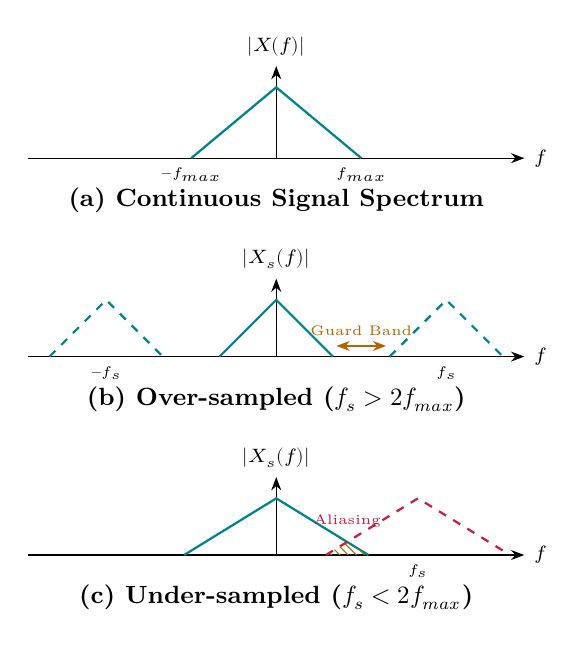
\begin{tikzpicture}[scale=0.9]
  % Axes for (a) Original Spectrum
  \draw[-Stealth, thin] (-3.5, 0) -- (3.5, 0) node[right, font=\scriptsize] {$f$};
  \draw[-Stealth, thin] (0, 0) -- (0, 1.3) node[above, font=\scriptsize] {$|X(f)|$};
  \draw[thick, color=myteal] (-1.2, 0) -- (0, 1.0) -- (1.2, 0);
  \node[below, font=\tiny] at (1.2, 0) {$f_{max}$};
  \node[below, font=\tiny] at (-1.2, 0) {$-f_{max}$};
  \node[font=\small\bfseries] at (0, -0.6) {(a) Continuous Signal Spectrum};

  % Axes for (b) Sampled Spectrum (No Aliasing)
  \begin{scope}[yshift=-2.8cm]
    \draw[-Stealth, thin] (-3.5, 0) -- (3.5, 0) node[right, font=\scriptsize] {$f$};
    \draw[-Stealth, thin] (0, 0) -- (0, 1.1) node[above, font=\scriptsize] {$|X_s(f)|$};
    % Center
    \draw[thick, color=myteal] (-0.8, 0) -- (0, 0.8) -- (0.8, 0);
    % Right replica
    \draw[thick, color=myteal, dashed] (1.6, 0) -- (2.4, 0.8) -- (3.2, 0);
    \node[below, font=\tiny] at (2.4, 0) {$f_s$};
    % Left replica
    \draw[thick, color=myteal, dashed] (-3.2, 0) -- (-2.4, 0.8) -- (-1.6, 0);
    \node[below, font=\tiny] at (-2.4, 0) {$-f_s$};
    % Guard band
    \draw[Stealth-Stealth, thin, color=myamber] (0.85, 0.15) -- (1.55, 0.15);
    \node[above, font=\tiny\color{myamber}] at (1.2, 0.15) {Guard Band};
    \node[font=\small\bfseries] at (0, -0.6) {(b) Over-sampled ($f_s > 2f_{max}$)};
  \end{scope}

  % Axes for (c) Aliased Spectrum
  \begin{scope}[yshift=-5.6cm]
    \draw[-Stealth, thin] (-3.5, 0) -- (3.5, 0) node[right, font=\scriptsize] {$f$};
    \draw[-Stealth, thin] (0, 0) -- (0, 1.1) node[above, font=\scriptsize] {$|X_s(f)|$};
    % Center
    \draw[thick, color=myteal] (-1.3, 0) -- (0, 0.8) -- (1.3, 0);
    % Right replica
    \draw[thick, color=myred, dashed] (0.7, 0) -- (2.0, 0.8) -- (3.3, 0);
    \node[below, font=\tiny] at (2.0, 0) {$f_s$};
    % Overlap region shading
    \fill[pattern=north west lines, pattern color=myamber] (0.7, 0) -- (1.0, 0.18) -- (1.3, 0) -- cycle;
    \node[above, font=\tiny\color{myred}] at (1.0, 0.25) {Aliasing};
    \node[font=\small\bfseries] at (0, -0.6) {(c) Under-sampled ($f_s < 2f_{max}$)};
  \end{scope}
\end{tikzpicture}
\end{tcolorbox}

\subsection{Signal Reconstruction}
Reconstruction is the process of converting discrete samples back into a continuous-time signal. Mathematically, this is done by passing the impulse train through an ideal low-pass filter (cutoff $f_c = f_s/2$). In time domain, this corresponds to the Whittaker-Shannon interpolation formula:
\[
x_a(t) = \sum_{n=-\infty}^{\infty} x(n) \text{sinc}\left(\frac{t - nT_s}{T_s}\right)
\]
In practice, a non-ideal \textbf{Zero-Order Hold (ZOH)} is used, which introduces a frequency roll-off governed by the $\text{sinc}(f/f_s)$ function, requiring a post-reconstruction smoothing filter.

% ===============================================================================
\section{Analog Continuous-Time Filters}
% ===============================================================================

\begin{tcolorbox}[defbox, title={\textbf{Butterworth vs. Chebyshev Filters}}]
\begin{itemize}[leftmargin=*, itemsep=2pt, topsep=0pt]
  \item \textbf{Butterworth Filter:} Characterized by a \textbf{maximally flat} magnitude response in the passband. The transfer function has only poles (no zeros). The magnitude squared is $|H(j\omega)|^2 = 1 / [1 + (\omega/\omega_c)^{2N}]$.
  \item \textbf{Chebyshev Filter (Type I):} Permits \textbf{equiripple behavior} in the passband to achieve a sharper transition band (faster roll-off) for the same filter order $N$.
\end{itemize}
\end{tcolorbox}

\subsection{Passive RC and RL Filters}
A passive filter uses only resistors, capacitors, and inductors. No power supply is needed, but no gain is possible. Passive filters are commonly used as anti-aliasing front-ends before ADC inputs.

\begin{tcolorbox}[formulabox, title={\textbf{First-Order Passive Filter Transfer Functions}}]
\textbf{RC Low-Pass Filter} (series $R$, shunt $C$):
\[
H_{LP}(s) = \frac{1/sC}{R + 1/sC} = \frac{\omega_c}{s + \omega_c} \qquad \omega_c = \frac{1}{RC}
\]
\textbf{RC High-Pass Filter} (series $C$, shunt $R$):
\[
H_{HP}(s) = \frac{R}{R + 1/sC} = \frac{s}{s + \omega_c}
\]
\textbf{RL Low-Pass Filter} (series $R$, shunt $L$):
\[
H_{LP}(s) = \frac{sL}{R + sL} \rightarrow \frac{\omega_c}{s + \omega_c} \qquad \omega_c = \frac{R}{L}
\]
Roll-off rate: $-20\,$dB/decade per filter order. At $\omega = \omega_c$: $|H| = 1/\sqrt{2}$ ($-3\,$dB point).
\end{tcolorbox}

\textbf{Limitations of Passive Filters:}
\begin{itemize}[leftmargin=*, itemsep=2pt]
  \item \textbf{Insertion Loss:} Even in the passband, passive filters attenuate the signal (no gain possible).
  \item \textbf{Loading Effect:} Connecting a load changes the effective cutoff frequency unless a buffer is added.
  \item \textbf{Slow Roll-off:} Only $-20\,$dB/decade per order; higher-order cascaded passive stages are impractical.
\end{itemize}
Active filters (Sallen-Key, Tow-Thomas) solve these limitations using op-amps for isolation and gain.

\subsection{Sallen-Key Active Biquad Filter}
The Sallen-Key is a popular second-order active filter stage (biquad). It uses a single operational amplifier configured as a voltage follower (gain $K \ge 1$) and two RC sections.

\begin{tcolorbox}[tikzbox, title={Second-Order Sallen-Key Low-Pass Active Filter}]
\centering
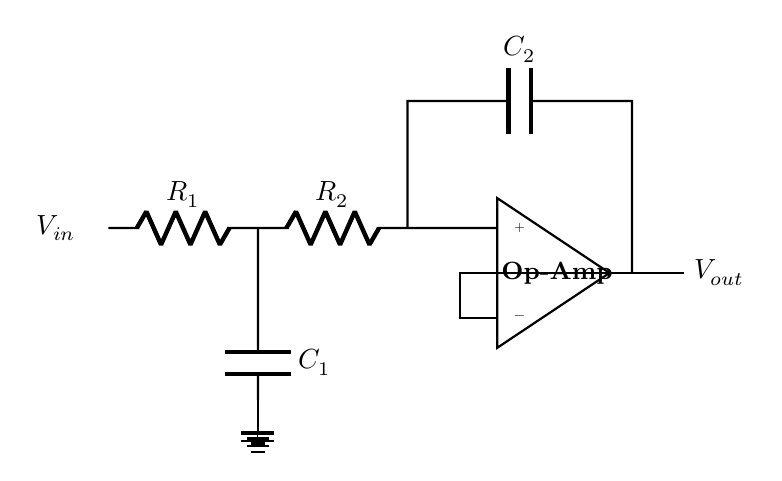
\begin{tikzpicture}[scale=0.95]
  % Op-amp
  \draw[thick] (4, 0.5) -- (4, -1.5) -- (5.5, -0.5) -- cycle;
  \node[font=\tiny] at (4.3, 0.1) {$+$};
  \node[font=\tiny] at (4.3, -1.1) {$-$};
  \node[font=\small\bfseries] at (4.8, -0.5) {Op-Amp};
  \draw[thick] (5.5, -0.5) -- (6.5, -0.5) node[right] {$V_{out}$};

  % Input branch
  \node[left] at (-1.5, 0.1) {$V_{in}$};
  \draw[thick] (-1.2, 0.1) to[R, l=$R_1$] (0.8, 0.1) to[R, l=$R_2$] (2.8, 0.1) -- (4.0, 0.1);
  \draw[thick] (0.8, 0.1) -- (0.8, -1.2) to[C, l=$C_1$] (0.8, -2.2) node[ground] {};
  \draw[thick] (2.8, 0.1) -- (2.8, 1.8) to[C, l=$C_2$] (5.8, 1.8) -- (5.8, -0.5);

  % Feedback and follower gain loop
  \draw[thick] (4.0, -1.1) -- (3.5, -1.1) -- (3.5, -0.5) -- (5.8, -0.5);
  \node[ground] at (0.8, -2.3) {};
\end{tikzpicture}
\end{tcolorbox}

For the Sallen-Key low-pass filter with $R_1 = R_2 = R$ and $C_1 = C_2 = C$ and unity amplifier gain ($K=1$):
\begin{tcolorbox}[formulabox, title={\textbf{Sallen-Key Transfer Function and Parameters}}]
\[
H(s) = \frac{V_{out}(s)}{V_{in}(s)} = \frac{1}{s^2 R^2 C^2 + 2sRC + 1}
\]
Comparing with the standard second-order biquad form $H(s) = \frac{\omega_0^2}{s^2 + \frac{\omega_0}{Q}s + \omega_0^2}$:
\[
\omega_0 = \frac{1}{RC} \qquad \text{(resonant angular frequency)}
\]
\[
Q = \frac{1}{2} = 0.5 \qquad \text{(quality factor)}
\]
\end{tcolorbox}

\subsection{Tow-Thomas State-Variable Biquad Filter}
The Tow-Thomas biquad is a multi-op-amp active filter that is highly stable and easily tunable. It consists of an input summing integrator, a second integrator, and an inverting amplifier to complete the feedback loop.

The transfer function for the Tow-Thomas bandpass output is:
\[
H_{BP}(s) = -\frac{s \frac{1}{R_4 C_1}}{s^2 + s \frac{1}{R_1 C_1} + \frac{1}{R_2 R_3 C_1 C_2}}
\]
This topology allows independent tuning of the gain, frequency $\omega_0$, and quality factor $Q$.

\subsection{Active Gm-C Filters}
At high frequencies (where op-amp open-loop gain drops), active RC filters suffer. \textbf{Gm-C filters} replace resistors and op-amps with \textbf{Operational Transconductance Amplifiers (OTAs)} (which act as voltage-controlled current sources: $I_{out} = g_m V_{in}$) and capacitors.
\begin{itemize}[leftmargin=*, itemsep=2pt]
  \item \textbf{OTA Integrator:} Output current charges a capacitor: $V_{out} = \frac{I_{out}}{sC} = \frac{g_m}{sC} V_{in}$.
  \item \textbf{High-Frequency Tuning:} The transconductance $g_m$ is electronically tunable by adjusting the OTA bias current, allowing real-time frequency tuning.
\end{itemize}

% ===============================================================================
\section{Basics of Analog Discrete-Time Filters \& Z-Transform}
% ===============================================================================

\begin{tcolorbox}[defbox, title={\textbf{Discrete-Time Filter Definition}}]
A discrete-time filter processes sequence samples $x(n)$ to produce output samples $y(n)$. It is described by a linear constant-coefficient difference equation:
\[
y(n) = \sum_{i=0}^{M} b_i x(n-i) - \sum_{j=1}^{N} a_j y(n-j)
\]
\end{tcolorbox}

\subsection{Z-Transform and ROC}
The Z-transform is the discrete-time equivalent of the Laplace transform. For a sequence $x(n)$, it is defined as:
\[
X(z) = \mathcal{Z}\{x(n)\} = \sum_{n=-\infty}^{\infty} x(n) z^{-n}
\]
where $z = r e^{j\omega}$ is a complex variable. The \textbf{Region of Convergence (ROC)} is the set of values in the $z$-plane for which the summation converges.
\begin{itemize}[leftmargin=*, itemsep=2pt]
  \item \textbf{Causal sequence:} ROC is the exterior of a circle ($|z| > R_{max}$).
  \item \textbf{Stable system:} The ROC must contain the unit circle ($|z| = 1$). This implies all poles of the system transfer function $H(z)$ must lie strictly inside the unit circle ($|poles| < 1$).
\end{itemize}

\subsection{Mapping s-Plane to z-Plane}
To design discrete-time filters from continuous-time templates, the s-plane must be mapped to the z-plane.
\begin{enumerate}[label=\textbf{\arabic*.}, leftmargin=*, itemsep=3pt]
  \item \textbf{Impulse Invariance:} Preserves the impulse response shape. The mapping is $z = e^{sT_s}$. This suffers from severe spectral aliasing.
  \item \textbf{Bilinear Transformation (BLT):} Maps the entire left half of the s-plane to the inside of the unit circle in the z-plane. It is defined by the algebraic mapping:
  \[
  s = \frac{2}{T_s} \frac{z - 1}{z + 1} \quad \Rightarrow \quad z = \frac{1 + s T_s/2}{1 - s T_s/2}
  \]
\end{enumerate}

\subsection{Frequency Warping Effect}
The BLT maps the infinite continuous frequency axis $-\infty < \Omega < \infty$ non-linearly to the finite discrete frequency axis $-\pi/T_s < \omega < \pi/T_s$. Substituting $s = j\Omega$ and $z = e^{j\omega T_s}$ gives the frequency relation:
\begin{tcolorbox}[formulabox, title={\textbf{Frequency Warping and Pre-warping Relations}}]
\[
\Omega = \frac{2}{T_s} \tan\left(\frac{\omega T_s}{2}\right)
\]
To compensate for this non-linear compression (warping), continuous-time specifications must be \textbf{pre-warped} before applying the BLT:
\[
\Omega_{pre} = \frac{2}{T_s} \tan\left(\frac{\omega_{desired} T_s}{2}\right)
\]
\end{tcolorbox}

\begin{tcolorbox}[examplebox, title={\textbf{Worked Example: Bilinear Transformation with Pre-warping}}]
\textbf{Problem:} Design a discrete low-pass filter with cutoff $f_d = 2\,$kHz at sampling rate $f_s = 10\,$kHz. Use a first-order continuous-time prototype $H(s) = \frac{\Omega_c}{s + \Omega_c}$.

\textbf{Solution:}
\begin{enumerate}[label=\textbf{\alph*.}, leftmargin=*, itemsep=2pt]
  \item Calculate $T_s = 1/f_s = 10^{-4}\,$s.
  \item Discrete angular frequency $\omega_d = 2\pi f_d = 4000\pi\,\text{rad/s}$.
  \item Pre-warped continuous frequency $\Omega_c$:
    \[
    \Omega_c = \frac{2}{10^{-4}} \tan\left(\frac{4000\pi \times 10^{-4}}{2}\right) = 20000 \tan(0.2\pi) \approx 20000 \times 0.7265 = 14530\,\text{rad/s}
    \]
  \item Apply Bilinear Transformation:
    \[
    H(z) = \left. \frac{\Omega_c}{s + \Omega_c} \right|_{s = \frac{2}{T_s}\frac{z-1}{z+1}} = \frac{14530}{\frac{2}{10^{-4}}\frac{z-1}{z+1} + 14530} = \frac{14530(z+1)}{20000(z-1) + 14530(z+1)}
    \]
    \[
    H(z) \approx \frac{14530(z+1)}{34530 z - 5470} \approx \frac{0.42(z+1)}{z - 0.158}
    \]
\end{enumerate}
\end{tcolorbox}

% ===============================================================================
% QUICK REVISION PAGE
% ===============================================================================
\newpage
\begin{center}
  {\large\bfseries\color{myred} Quick Revision --- Module 1}\\[3pt]
  {\small\color{mydark} Filter Fundamentals and Z-Transform $|$ PE-EC802A}
\end{center}
\noindent{\color{myred}\rule{\linewidth}{1.2pt}}
\vspace{4pt}

\begin{tcolorbox}[formulabox, title={\textbf{Key Formulas and Transforms at a Glance}}]
\renewcommand{\arraystretch}{1.35}
\begin{tabularx}{\linewidth}{B{5.0cm} X}
Nyquist Sampling Rate & $f_s \ge 2 f_{max}$ \\[4pt]
Sinc Reconstruction & $x_a(t) = \sum x(n) \text{sinc}\left(\frac{t - nT_s}{T_s}\right)$ \\[4pt]
Sallen-Key LP frequency & $\omega_0 = \frac{1}{\sqrt{R_1 R_2 C_1 C_2}}$; \quad $Q = \frac{\sqrt{R_1 R_2 C_1 C_2}}{R_1 C_2 + R_2 C_2 + (1-K)R_1 C_1}$ \\[4pt]
Bilinear Transformation & $s = \frac{2}{T_s} \frac{z-1}{z+1}$ \\[4pt]
Frequency Warping relation & $\Omega = \frac{2}{T_s} \tan\left(\frac{\omega T_s}{2}\right)$ \\[4pt]
Z-transform & $X(z) = \sum_{n=-\infty}^{\infty} x(n) z^{-n}$ \\[4pt]
Unit circle frequency map & $z = e^{j\omega T_s}$ \\[4pt]
\end{tabularx}
\end{tcolorbox}

\begin{tcolorbox}[defbox, title={\textbf{One-Line Definitions}}]
\begin{itemize}[leftmargin=*, itemsep=2pt, topsep=0pt]
  \item \textbf{Aliasing:} High frequencies folding back to lower bands due to under-sampling ($f_s < 2f_{max}$).
  \item \textbf{Anti-Aliasing Filter:} A low-pass filter limiting analog signal bandwidth to $f_s/2$ before sampling.
  \item \textbf{Butterworth Response:} Maximally flat magnitude profile in the passband.
  \item \textbf{Chebyshev Response:} Passband equiripple profile resulting in a sharper cutoff transition band.
  \item \textbf{Biquad Filter:} A second-order active filter block implementing a pair of poles and optionally zeros.
  \item \textbf{Gm-C Filter:} A high-frequency filter using transconductance amplifiers and capacitors.
  \item \textbf{ROC:} The region in the z-plane where the Z-transform power series converges.
  \item \textbf{Frequency Warping:} Nonlinear compression of the continuous frequency axis introduced by the bilinear transformation.
\end{itemize}
\end{tcolorbox}

\begin{tcolorbox}[tikzbox, title={\textbf{Analog Filter Topology Comparison}}]
\centering
\par\noindent
\renewcommand{\arraystretch}{1.3}
\begin{tabularx}{\linewidth}{|B{2.6cm}|Y|Y|Y|}
\hline
\textbf{Type} & \textbf{Active Elements} & \textbf{Key Property} & \textbf{Use Case} \\ \hline
\textbf{Passive RC/RL} & None & No gain, simple & AAF, RF matching \\ \hline
\textbf{Butterworth} & Op-amp & Maximally flat passband & General purpose LP \\ \hline
\textbf{Chebyshev} & Op-amp & Equiripple, sharp cutoff & Steeper rolloff needed \\ \hline
\textbf{Sallen-Key} & 1 op-amp & 2nd-order, easy design & Active LP/HP/BP \\ \hline
\textbf{Tow-Thomas} & 3 op-amps & Tunable $\omega_0$, $Q$ & Precision biquad \\ \hline
\textbf{Gm-C} & OTA (no R) & High-freq, tunable & $>100\,$MHz filters \\ \hline
\end{tabularx}
\end{tcolorbox}

\begin{tcolorbox}[exambox, title={\textbf{Frequently Asked / Viva Questions}}]
\begin{enumerate}[topsep=0pt, label=\textbf{Q\arabic*.}, itemsep=5pt]
  \item \Q{State the sampling theorem. What happens if the sampling rate is below the Nyquist rate?}
    The sampling theorem states that the sampling rate $f_s$ must be at least twice the maximum signal frequency component ($f_s \ge 2 f_{max}$). Under-sampling causes high frequencies to overlap with low frequencies, creating irreversible aliasing distortion.
  \item \Q{What is the function of the anti-aliasing filter?}
    It is an analog low-pass filter placed before the sampler to block all frequency components above $f_s/2$, ensuring the sampling condition is satisfied.
  \item \Q{Compare Butterworth and Chebyshev filter characteristics.}
    Butterworth filters are maximally flat in the passband but have a slower roll-off. Chebyshev filters have equiripple passband characteristics and a much steeper roll-off transition band.
  \item \Q{Explain the Sallen-Key active filter configuration.}
    It is a second-order active filter structure using one operational amplifier configured as a voltage follower, providing high input impedance, low output impedance, and easily calculable components.
  \item \Q{What are the advantages of Gm-C filters over active RC filters?}
    Gm-C filters do not need operational amplifiers or resistors. They use transconductance amplifiers (OTAs) and capacitors, making them suitable for high-frequency operation (up to hundreds of MHz) and electronically tunable.
  \item \Q{Why does the bilinear transformation map the left half of the s-plane to the inside of the z-plane unit circle?}
    The BLT maps $s = \sigma + j\Omega$ using $z = (1+sT/2)/(1-sT/2)$. For $\sigma < 0$ (LHP), the numerator magnitude is smaller than the denominator magnitude, ensuring $|z| < 1$ (inside the unit circle).
  \item \Q{What is frequency warping in the Bilinear Transformation, and how is it compensated?}
    It is the non-linear compression of the continuous frequency axis $\Omega$ to the discrete axis $\omega$. It is compensated by pre-warping continuous-time critical frequencies: $\Omega_c = \frac{2}{T_s}\tan(\omega_d T_s /2)$.
  \item \Q{State the condition for a discrete-time LTI system to be stable.}
    The system is stable if its Z-transform region of convergence (ROC) contains the unit circle ($|z|=1$), which requires all poles to lie strictly inside the unit circle.
  \item \Q{What is the Z-transform of a causal sequence $a^n u(n)$? State its ROC.}
    The Z-transform is $H(z) = \frac{z}{z-a}$ (or $\frac{1}{1-a z^{-1}}$) with the region of convergence $|z| > |a|$.
  \item \Q{Why is the impulse invariance mapping not suitable for high-pass and band-stop filters?}
    Impulse invariance maps frequencies linearly, which causes severe aliasing at high frequencies. High-pass and band-stop filters have infinite high-frequency energy, making aliasing unacceptable.
\end{enumerate}
\end{tcolorbox}


% -- Module 2 -----------------------------------------------------------------
\modulestart{2}{Switched-Capacitor (SC) Circuits \& Resistor Equivalence}

\section{Switched-Capacitor (SC) Circuits \& Resistor Equivalence}
% ===============================================================================

\begin{tcolorbox}[defbox, title={\textbf{Switched-Capacitor Circuit Concept}}]
A \textbf{Switched-Capacitor (SC) circuit} is a discrete-time signal processing circuit that implements resistors by rapidly switching charge back and forth between capacitors using non-overlapping clock phases. SC circuits are highly preferred in CMOS technology because precise on-chip resistors are difficult to fabricate, whereas capacitor ratios can be matched with extremely high accuracy (up to $0.1\%$).
\end{tcolorbox}

\subsection{Switched-Capacitor Filter Architectures}
A practical SC biquad (second-order section) is built using two SC integrators in a feedback loop. The \textbf{Fleischer-Laker biquad} is the standard SC biquad implementing LP, HP, and BP outputs simultaneously.

\begin{tcolorbox}[tikzbox, title={Fleischer-Laker SC Biquad Block Structure}]
\centering
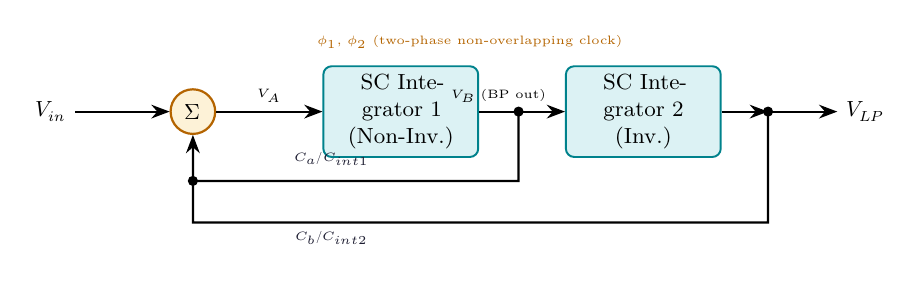
\begin{tikzpicture}[scale=0.88, transform shape]
  % Two SC integrator blocks
  \node[block, text width=2.0cm] (int1) at (1.5, 0) {SC Integrator 1\\ (Non-Inv.)};
  \node[block, text width=2.0cm] (int2) at (5.0, 0) {SC Integrator 2\\ (Inv.)};
  \node[sumjunc] (sum) at (-1.5, 0) {$\Sigma$};

  % Forward path
  \draw[-Stealth, thick] (sum.east) -- (int1.west) node[midway, above, font=\tiny]{$V_A$};
  \draw[thick] (int1.east) -- (3.2, 0) node[midway, above, font=\tiny]{$V_B$ (BP out)};
  \draw[-Stealth, thick] (3.2, 0) -- (int2.west);
  \draw[-Stealth, thick] (int2.east) -- (6.8, 0);
  \draw[-Stealth, thick] (6.8, 0) -- (7.8, 0) node[right, font=\small]{$V_{LP}$};

  % Feedback paths
  \draw[thick] (6.8, 0) to[short, *-] (6.8, -1.6) -- (-1.5, -1.6) -- (-1.5, -1.0);
  \draw[thick] (3.2, 0) to[short, *-] (3.2, -1.0) to[short, -*] (-1.5, -1.0);
  \draw[-Stealth, thick] (-1.5, -1.0) -- (sum.south);

  % Input
  \draw[-Stealth, thick] (-3.2, 0) node[left, font=\small]{$V_{in}$} -- (sum.west);

  % Capacitor ratio labels on feedback
  \node[above, font=\tiny\color{mydark}] at (0.5, -0.9) {$C_a/C_{int1}$};
  \node[below, font=\tiny\color{mydark}] at (0.5, -1.6) {$C_b/C_{int2}$};

  % Clock label
  \node[font=\tiny, color=myamber] at (2.5, 1.0) {$\phi_1$, $\phi_2$ (two-phase non-overlapping clock)};
\end{tikzpicture}
\end{tcolorbox}

\textbf{How the Fleischer-Laker Biquad Sets Frequency and Q:}
\begin{itemize}[leftmargin=*, itemsep=2pt]
  \item Pole frequency: $\omega_0 \propto \frac{f_{clk} \cdot C_{sampling}}{C_{integrating}}$ --- set purely by capacitor ratios and clock frequency.
  \item Quality factor $Q$: set by the feedback capacitor ratio. Changing $C_a$ and $C_b$ independently controls $\omega_0$ and $Q$ without interaction.
\end{itemize}

\subsection{Switched-Capacitor Filter Applications}
\begin{itemize}[leftmargin=*, itemsep=2.5pt]
  \item \textbf{Audio CODEC:} Anti-aliasing and reconstruction filters in 16--24-bit audio codecs (e.g., CD player, smartphone DAC) where precise $\pm 0.01\%$ corner frequency tolerance is required.
  \item \textbf{$\Delta\Sigma$ ADC Front-End:} SC integrators inside $\Delta\Sigma$ modulators perform the summation and integration operations that shape quantization noise to high frequencies.
  \item \textbf{DTMF (Dual-Tone Multi-Frequency) Decoding:} Narrow-band bandpass SC filters detect individual telephone dial tones.
  \item \textbf{Biomedical Instrumentation:} Low-frequency, high-accuracy SC filters for ECG/EEG signal conditioning, where process-insensitive frequency accuracy is essential.
\end{itemize}

\subsection{Derivation of SC Resistor Equivalence}
Consider a capacitor $C$ connected between two voltage nodes $V_1$ and $V_2$ via two single-pole single-throw switches controlled by non-overlapping clock phases $\Phi_1$ and $\Phi_2$ with a clock frequency $f_c = 1/T_c$.

\begin{tcolorbox}[tikzbox, title={Switched-Capacitor Resistor Equivalence Circuit}]
\centering
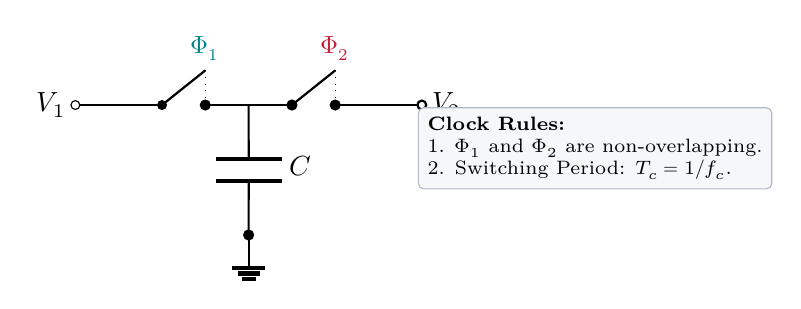
\begin{tikzpicture}[scale=1.1]
  % Nodes
  \draw (0,0) node[left] {$V_1$} to[short, o-*] (1,0);
  
  % Switch 1 (Phi 1)
  \draw[thick] (1,0) -- (1.5,0.4) node[above, font=\small\color{myteal}] {$\Phi_1$};
  \draw[dotted] (1.5,0.4) -- (1.5,0);
  \draw[thick] (1.5,0) to[short, *-*] (2.5,0);
  
  % Switch 2 (Phi 2)
  \draw[thick] (2.5,0) -- (3.0,0.4) node[above, font=\small\color{myred}] {$\Phi_2$};
  \draw[dotted] (3.0,0.4) -- (3.0,0);
  \draw[thick] (3.0,0) to[short, *-o] (4.0,0) node[right] {$V_2$};
  
  % Capacitor
  \draw[thick] (2.0,0) to[C, l=$C$, -*] (2.0,-1.5) node[ground] {};
  
  % Timing diagram / Clock phase labeling
  \node[draw=mgframe, fill=mygray, rounded corners=2pt, font=\scriptsize, align=left] at (6.0,-0.5) {
    \textbf{Clock Rules:}\\
    1. $\Phi_1$ and $\Phi_2$ are non-overlapping.\\
    2. Switching Period: $T_c = 1/f_c$.
  };
\end{tikzpicture}
\end{tcolorbox}

\textbf{Step-by-step Derivation:}
\begin{enumerate}[label=\textbf{\arabic*.}, leftmargin=*, itemsep=3pt]
  \item During phase $\Phi_1$, Switch 1 is closed and Switch 2 is open. The capacitor $C$ charges to voltage $V_1$.
  The charge stored on the capacitor is:
  \[
  Q_1 = C V_1
  \]
  \item During phase $\Phi_2$, Switch 1 opens and Switch 2 closes. The capacitor $C$ is connected to $V_2$, charging or discharging to $V_2$.
  The charge remaining on the capacitor is:
  \[
  Q_2 = C V_2
  \]
  \item The net charge transferred from node $V_1$ to node $V_2$ in one clock period $T_c$ is:
  \[
  \Delta Q = Q_1 - Q_2 = C(V_1 - V_2)
  \]
  \item The average current $I_{avg}$ flowing from node $V_1$ to node $V_2$ is the charge transferred per unit time:
  \[
  I_{avg} = \frac{\Delta Q}{T_c} = \frac{C(V_1 - V_2)}{T_c} = f_c C (V_1 - V_2)
  \]
  \item Using Ohm's Law ($I = \frac{V_1 - V_2}{R_{eq}}$), we find the equivalent resistance $R_{eq}$ of the switched-capacitor stage:
  \begin{tcolorbox}[formulabox, title={\textbf{SC Equivalent Resistance}}]
  \[
  R_{eq} = \frac{V_1 - V_2}{I_{avg}} = \frac{1}{f_c C}
  \]
  where:
  \begin{itemize}[leftmargin=1.5em, itemsep=1pt]
    \item $R_{eq} = $ Equivalent resistance ($\Omega$)
    \item $f_c = $ Clock switching frequency (Hz)
    \item $C = $ Capacitance (F)
  \end{itemize}
  \end{tcolorbox}
\end{enumerate}

\subsection{Significance of SC Circuits in IC Design}
In integrated circuits, fabricating large resistors (e.g., $100\,$k$\Omega$) is highly impractical because:
\begin{itemize}[leftmargin=*, itemsep=2pt]
  \item \textbf{Area:} Polysilicon/diffusion resistors require massive silicon area.
  \item \textbf{Accuracy:} Absolute tolerances of resistors on silicon are poor ($\pm 20\%$) and drift significantly with temperature.
  \item \textbf{Tuning:} RC time constants ($\tau = RC$) vary by up to $40\%$ due to process variations.
\end{itemize}
In contrast, in SC circuits, the equivalent time constant of an integrator is:
\[
\tau = R_{eq} C_2 = \left(\frac{1}{f_c C_1}\right) C_2 = \frac{1}{f_c} \left(\frac{C_2}{C_1}\right)
\]
Since $f_c$ is derived from a highly stable crystal oscillator and $\frac{C_2}{C_1}$ is a ratio of two matched capacitors (which matches perfectly within $0.1\%$ on layout), the time constant $\tau$ is extremely accurate and temperature-independent.

% ===============================================================================
\section{SC Non-Idealities \& Mitigation Strategies}
% ===============================================================================

In real CMOS processes, MOS transistors act as non-ideal switches. The key non-idealities are:

\subsection{1. Charge Injection}
When a MOS switch is turned ON, a channel charge $Q_{ch}$ is accumulated in the inversion layer:
\[
Q_{ch} = W L C_{ox} (V_{GS} - V_{TH}) = W L C_{ox} (V_{CLK} - V_{in} - V_{TH})
\]
When the switch is turned OFF (gate voltage drops), this channel charge is released and flows out through the source and drain terminals. The charge injected into the sampling capacitor $C$ shifts the sampled voltage, introducing an offset and non-linear distortion (since $V_{TH}$ depends non-linearly on $V_{in}$ via the body effect).

\subsection{2. Clock Feedthrough}
The overlap capacitance $C_{ov}$ between the gate and source/drain terminals forms a capacitive voltage divider with the sampling capacitor. The clock transition at the gate is directly coupled to the sampling capacitor:
\[
\Delta V = V_{CLK} \left( \frac{C_{ov}}{C_{ov} + C} \right)
\]
This introduces a constant offset voltage to the sampled signal.

\subsection{3. thermal Noise ($k_B T / C$ Noise)}
An ON transistor has a finite channel resistance $R_{on}$. This resistance generates thermal noise with a power spectral density of $4 k_B T R_{on}$. When the switch is opened, this noise is sampled onto the capacitor. The total noise power integrated over the loop bandwidth is:
\begin{tcolorbox}[formulabox, title={\textbf{Thermal Noise Limit (kT/C)}}]
\[
v_n^2 = \int_0^{\infty} \frac{4 k_B T R_{on}}{1 + (2\pi f R_{on} C)^2} df = \frac{k_B T}{C}
\]
where $k_B$ is the Boltzmann constant ($1.38 \times 10^{-23}$ J/K) and $T$ is temperature in Kelvin.
\end{tcolorbox}
This noise sets a fundamental limit on the dynamic range (SNDR) of switched-capacitor circuits. To achieve higher resolution, $C$ must be made larger, which increases power consumption and area.

\begin{tcolorbox}[tikzbox, title={Summary of Switch Mitigation Techniques}]
\centering
\par\noindent
\begin{tabularx}{\linewidth}{|B{3.5cm}|Y|Y|}
\hline
\textbf{Non-Ideality} & \textbf{Physical Mechanism} & \textbf{Mitigation Strategy} \\ \hline
\textbf{Charge Injection} & Channel charge flows into $C$ upon turn-off & Dummy switches, differential signaling, bottom-plate sampling \\ \hline
\textbf{Clock Feedthrough} & Overlap capacitance $C_{ov}$ couples clock edges & CMOS transmission gates, differential architectures \\ \hline
\textbf{Thermal Noise} & Thermal noise of $R_{on}$ is sampled onto $C$ & Increase capacitance value $C$ ($v_n \propto 1/\sqrt{C}$) \\ \hline
\end{tabularx}
\end{tcolorbox}

% ===============================================================================
\section{Stray-Insensitive Integrators}
% ===============================================================================

Early SC designs were sensitive to parasitic capacitances between node terminals and substrate (ground), causing gain errors. Modern SC systems use \textbf{stray-insensitive} configurations.

\subsection{Stray-Insensitive Non-Inverting Integrator}
The stray-insensitive non-inverting integrator uses 4 switches controlled by non-overlapping clocks $\Phi_1$ and $\Phi_2$.

\begin{tcolorbox}[tikzbox, title={Stray-Insensitive Non-Inverting SC Integrator Circuit}]
\centering
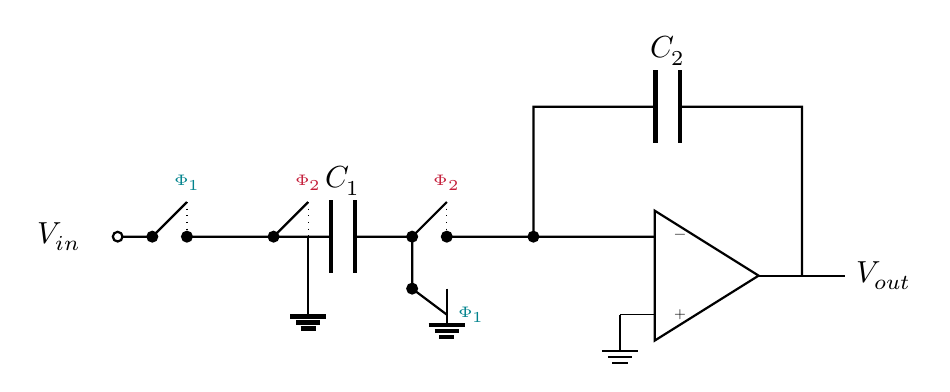
\begin{tikzpicture}[scale=1.1, transform shape]
  % Op-amp
  \draw[thick] (5, 0) -- (5, -1.5) -- (6.2, -0.75) -- cycle;
  \node[font=\tiny] at (5.3, -0.3) {$-$};
  \node[font=\tiny] at (5.3, -1.2) {$+$};
  \draw (5, -1.2) -- (4.6, -1.2) node[ground] {};
  \draw[thick] (6.2, -0.75) -- (7.2, -0.75) node[right] {$V_{out}$};

  % Input node and switches
  \node[left] at (-1.5, -0.3) {$V_{in}$};
  \draw[thick] (-1.2, -0.3) to[short, o-*] (-0.8, -0.3);
  
  % Switch S1 (Phi 1)
  \draw[thick] (-0.8, -0.3) -- (-0.4, 0.1) node[above, font=\tiny\color{myteal}] {$\Phi_1$};
  \draw[dotted] (-0.4, 0.1) -- (-0.4, -0.3);
  \draw[thick] (-0.4, -0.3) to[short, *-*] (0.6, -0.3);

  % Switch S2 (Phi 2)
  \draw[thick] (0.6, -0.3) -- (1.0, 0.1) node[above, font=\tiny\color{myred}] {$\Phi_2$};
  \draw[dotted] (1.0, 0.1) -- (1.0, -0.3);
  \draw[thick] (1.0, -0.3) -- (1.0, -0.8) node[ground] {};

  % Input Capacitor C1
  \draw[thick] (0.6, -0.3) to[C, l=$C_1$, -*] (2.2, -0.3);

  % Switch S3 (Phi 2)
  \draw[thick] (2.2, -0.3) -- (2.6, 0.1) node[above, font=\tiny\color{myred}] {$\Phi_2$};
  \draw[dotted] (2.6, 0.1) -- (2.6, -0.3);
  \draw[thick] (2.6, -0.3) to[short, *-*] (3.6, -0.3) -- (5, -0.3);

  % Switch S4 (Phi 1)
  \draw[thick] (2.2, -0.3) -- (2.2, -0.8) to[short, -*] (2.2, -0.9);
  \draw[thick] (2.2, -0.9) -- (2.6, -1.2) node[right, font=\tiny\color{myteal}] {$\Phi_1$};
  \draw[dotted] (2.6, -1.2) -- (2.6, -0.9);
  \draw[thick] (2.6, -0.9) node[ground] {};

  % Feedback Capacitor C2
  \draw[thick] (3.6, -0.3) -- (3.6, 1.2) to[C, l=$C_2$] (6.7, 1.2) -- (6.7, -0.75);
  \draw[thick] (6.7, -0.75) -- (6.2, -0.75);
\end{tikzpicture}
\end{tcolorbox}

\textbf{Analysis of Stray Insensitivity:}
\begin{itemize}[leftmargin=*, itemsep=2.5pt]
  \item \textbf{Node A (left plate of $C_1$):} Connected to either $V_{in}$ (low impedance source) during $\Phi_1$ or to ground during $\Phi_2$. Any parasitic capacitor at this node is either charged by $V_{in}$ or fully discharged to ground, never affecting the charge transferred to the integrating capacitor $C_2$.
  \item \textbf{Node B (right plate of $C_1$):} Connected to virtual ground (op-amp inverting terminal) during $\Phi_2$ or to physical ground during $\Phi_1$. The potential is always at ground (virtual or physical), so the voltage across its parasitics is always $0\,$V. Thus, no charge is stored or injected by the parasitic capacitance.
\end{itemize}

\subsection{Charge Equations and Transfer Function}
Let us write the discrete-time charge conservation equation at the virtual ground node:
\begin{enumerate}[label=\textbf{\arabic*.}, leftmargin=*, itemsep=3pt]
  \item During $\Phi_1(n-1)$, $C_1$ charges to $V_{in}(n-1)$ (left terminal to $V_{in}$, right terminal to ground).
  \[
  q_{C1}(n-1) = C_1 V_{in}(n-1)
  \]
  \item During $\Phi_2(n)$, $C_1$ is connected to ground on the left and virtual ground on the right. The capacitor is fully discharged, and its charge flows entirely into $C_2$. The feedback capacitor $C_2$ accumulates this charge:
  \[
  C_2 V_{out}(n) = C_2 V_{out}(n-1) + C_1 V_{in}(n-1)
  \]
  \item Taking the Z-transform of this difference equation:
  \[
  C_2 Y(z) = C_2 z^{-1} Y(z) + C_1 z^{-1} X(z)
  \]
  \[
  Y(z)(1 - z^{-1}) = \frac{C_1}{C_2} z^{-1} X(z)
  \]
  \item The transfer function $H(z) = Y(z)/X(z)$ is:
  \begin{tcolorbox}[formulabox, title={\textbf{Non-Inverting SC Integrator Transfer Function}}]
  \[
  H(z) = \frac{V_{out}(z)}{V_{in}(z)} = \frac{C_1}{C_2} \frac{z^{-1}}{1 - z^{-1}}
  \]
  \end{tcolorbox}
  The term $z^{-1}$ in the numerator indicates a delay of one clock cycle, making this a \textbf{delaying (non-inverting) integrator}.
\end{enumerate}

If we modify the switch network such that $C_1$ is connected to $V_{in}$ and virtual ground during the same clock phase, we obtain an \textbf{inverting (non-delaying) integrator} with transfer function:
\[
H(z) = -\frac{C_1}{C_2} \frac{1}{1 - z^{-1}}
\]

% ===============================================================================
\section{First-Order \& Second-Order SC Filters (Biquads)}
% ===============================================================================

\subsection{Fleischer-Laker Biquad Topology}
The Fleischer-Laker biquad is a standard stray-insensitive second-order SC filter stage. It consists of two op-amps and a network of switched and unswitched capacitors. It can implement low-pass, high-pass, band-pass, and notch transfer functions by selecting appropriate capacitor ratios.

The general Z-domain transfer function of a second-order SC biquad is given by:
\[
H(z) = \frac{N(z)}{D(z)} = \frac{\alpha_0 + \alpha_1 z^{-1} + \alpha_2 z^{-2}}{1 + \beta_1 z^{-1} + \beta_2 z^{-2}}
\]
By mapping s-plane specifications (e.g. pole frequency $\omega_0$ and quality factor $Q$) through the Bilinear Transformation, the discrete coefficients $\alpha_i$ and $\beta_i$ are determined, allowing direct calculation of the required capacitor ratios.

% ===============================================================================
% QUICK REVISION PAGE
% ===============================================================================
\newpage
\begin{center}
  {\large\bfseries\color{myred} Quick Revision --- Module 2}\\[3pt]
  {\small\color{mydark} Switched-Capacitor Filters $|$ PE-EC802A}
\end{center}
\noindent{\color{myred}\rule{\linewidth}{1.2pt}}
\vspace{4pt}

\begin{tcolorbox}[formulabox, title={\textbf{Key Formulas at a Glance}}]
\renewcommand{\arraystretch}{1.35}
\begin{tabularx}{\linewidth}{B{5.0cm} X}
Equivalent Resistance & $R_{eq} = \frac{1}{f_c C}$ \\[4pt]
Integrator Time Constant & $\tau = \frac{1}{f_c} \left( \frac{C_2}{C_1} \right)$ \\[4pt]
Thermal Noise Power & $v_n^2 = \frac{k_B T}{C}$ \\[4pt]
Non-Inverting SC Integrator & $H(z) = \frac{C_1}{C_2} \frac{z^{-1}}{1 - z^{-1}}$ \\[4pt]
Inverting SC Integrator & $H(z) = -\frac{C_1}{C_2} \frac{1}{1 - z^{-1}}$ \\[4pt]
Channel Charge & $Q_{ch} = W L C_{ox}(V_{CLK} - V_{in} - V_{TH})$ \\[4pt]
Clock Feedthrough Offset & $\Delta V = V_{CLK} \left( \frac{C_{ov}}{C_{ov} + C} \right)$ \\
\end{tabularx}
\end{tcolorbox}

\begin{tcolorbox}[defbox, title={\textbf{One-Line Definitions}}]
\begin{itemize}[leftmargin=*, itemsep=2pt, topsep=0pt]
  \item \textbf{SC Resistor Equivalence:} A capacitor switched at high rate acts as a resistor of value $1/(f_c C)$.
  \item \textbf{Non-overlapping Clocks:} Clock signals $\Phi_1$ and $\Phi_2$ that are never high at the same time to prevent direct shorting.
  \item \textbf{Charge Injection:} Channel charge of a switching MOS transistor entering the sampling capacitor upon turn-off.
  \item \textbf{Clock Feedthrough:} Direct capacitive coupling of the clock transition to the node via overlap capacitance.
  \item \textbf{Stray-Insensitive Integrator:} SC integrator topology immune to parasitics of capacitors to substrate/ground.
  \item \textbf{kT/C Noise:} The fundamental thermodynamic limit on sampled voltage accuracy, equal to $k_B T / C$.
  \item \textbf{Stray-Insensitive SC Integrator:} An SC integrator topology where parasitic capacitances at the virtual ground node of the op-amp are shielded and do not contribute to the transfer function.
\end{itemize}
\end{tcolorbox}

\begin{tcolorbox}[tikzbox, title={\textbf{Continuous-Time vs.~Switched-Capacitor Filter Comparison}}]
\centering
\par\noindent
\renewcommand{\arraystretch}{1.3}
\begin{tabularx}{\linewidth}{|B{2.8cm}|Y|Y|}
\hline
\textbf{Property} & \textbf{Active RC Filter} & \textbf{Switched-Capacitor Filter} \\ \hline
\textbf{$\omega_c$ accuracy} & Depends on absolute $R$, $C$ ($\pm20\%$) & Set by $C$ ratio $\times$ $f_{clk}$ ($<0.1\%$) \\ \hline
\textbf{Tuning} & Manual trim required & Reprogram $f_{clk}$ \\ \hline
\textbf{Frequency range} & DC to $>1\,$GHz & DC to $\sim f_{clk}/2$ (audio/kHz range) \\ \hline
\textbf{Clock noise} & Not applicable & Clock feedthrough adds noise floor \\ \hline
\textbf{Silicon area} & Needs large R, C & Compact (capacitors only) \\ \hline
\textbf{CMOS compatible} & Requires resistors & Fully CMOS-compatible \\ \hline
\end{tabularx}
\end{tcolorbox}

\begin{tcolorbox}[exambox, title={\textbf{Frequently Asked / Viva Questions}}]
\begin{enumerate}[topsep=0pt, label=\textbf{Q\arabic*.}, itemsep=5pt]
  \item \Q{Derive the equivalent resistance of a switched capacitor.}
    A capacitor $C$ charged to $V_1$ at phase $\Phi_1$ holds charge $Q_1 = C V_1$. At phase $\Phi_2$, it discharges to $V_2$, holding charge $Q_2 = C V_2$. The net charge transferred per cycle is $\Delta Q = C(V_1-V_2)$. The average current is $I_{avg} = \Delta Q / T_c = f_c C (V_1-V_2)$. Since $R_{eq} = (V_1-V_2)/I_{avg}$, we get $R_{eq} = 1/(f_c C)$.
  \item \Q{Why are switched-capacitor circuits preferred over continuous-time active RC circuits on-chip?}
    Precise resistors are hard to fabricate in CMOS (requiring huge area and having $\pm 20\%$ variations). SC circuits replace resistors with capacitors. The time constant depends on the ratio of two matched capacitors, which matches within $0.1\%$, providing highly precise and temperature-stable performance.
  \item \Q{What is kT/C noise and what limits does it impose?}
    It is the thermal noise power sampled onto a capacitor from the switch channel resistance. It is independent of the switch resistance and equals $k_B T / C$. It sets a lower limit on signal resolution; higher dynamic range requires larger capacitors.
  \item \Q{Explain the mechanism of charge injection in MOS switches.}
    When an MOS transistor is ON, it has charge in its inversion channel. When it turns OFF, this charge exits through the source and drain terminals, injecting charge into the sampling capacitor, shifting the voltage and causing non-linear distortion.
  \item \Q{How does a dummy switch mitigate charge injection?}
    A dummy transistor (usually half the size of the main switch with source/drain shorted) is connected in series. It is driven by the complementary clock. When the main switch turns OFF and releases charge, the dummy switch turns ON and absorbs that charge, neutralizing the error.
  \item \Q{What is bottom-plate sampling, and why is it stray-insensitive?}
    It is a switching technique where the switch connected to the virtual ground (bottom plate) is opened slightly before the input switch. Since the bottom plate is at virtual ground, the charge injected is constant and independent of the input voltage, eliminating non-linear distortion.
  \item \Q{Show the Z-domain transfer function of a non-inverting SC integrator.}
    It is $H(z) = \frac{C_1}{C_2} \frac{z^{-1}}{1 - z^{-1}}$, which represents a delaying integrator.
  \item \Q{Compare inverting and non-inverting SC integrator transfer functions.}
    The inverting integrator is non-delaying: $H(z) = -\frac{C_1}{C_2} \frac{1}{1-z^{-1}}$. The non-inverting integrator has a delay: $H(z) = \frac{C_1}{C_2} \frac{z^{-1}}{1-z^{-1}}$.
  \item \Q{What is the Fleischer-Laker biquad?}
    It is a stray-insensitive, second-order switched-capacitor filter topology capable of implementing any generic second-order transfer function (LP, HP, BP, Notch) by choosing appropriate capacitor values.
  \item \Q{What is clock feedthrough and how is it reduced?}
    Clock feedthrough is the coupling of the clock gate signal to the sampling capacitor via the MOS gate-overlap capacitances. It is reduced by using transmission gates (where PMOS and NMOS cancel each other's transitions) or differential architectures.
\end{enumerate}
\end{tcolorbox}


% -- Module 3 -----------------------------------------------------------------
\modulestart{3}{Data Converter Performance Metrics}

\section{Data Converter Performance Metrics}
% ===============================================================================

Data converters form the bridge between the analog physical world and the digital processing domain. Their performance is specified by static and dynamic parameters.

\subsection{Static Metrics: DNL and INL}
Let $\Delta$ (or $1\,\text{LSB} = V_{FS}/2^N$) represent the ideal step size of the converter.

\begin{tcolorbox}[defbox, title={\textbf{Differential Non-Linearity (DNL)}}]
\textbf{Differential Non-Linearity (DNL)} measures the deviation of an actual step width from the ideal value of $1\,\text{LSB}$. For an ADC, it is the difference between the actual step width $W_k$ and the ideal $1\,\text{LSB}$:
\[
\text{DNL}_k = \frac{W_k - \text{LSB}}{\text{LSB}}
\]
If DNL becomes less than $-1\,\text{LSB}$, the step width becomes zero or negative, leading to \textbf{missing codes} in ADCs. A system is guaranteed monotonic if $\text{DNL} > -1\,\text{LSB}$.
\end{tcolorbox}

\begin{tcolorbox}[defbox, title={\textbf{Integral Non-Linearity (INL)}}]
\textbf{Integral Non-Linearity (INL)} measures the deviation of the actual transfer function characteristics from the straight line (ideal transfer curve) connecting the endpoints (zero-scale and full-scale). It represents the cumulative sum of DNL errors:
\[
\text{INL}_k = \sum_{i=1}^{k} \text{DNL}_i
\]
INL directly limits the harmonic distortion and linearity of the system.
\end{tcolorbox}

\subsection{Quantization Noise Derivation}
Quantization is the process of mapping a continuous range of values to a discrete set. The difference between the continuous input $x$ and its quantized representation $q(x)$ is the quantization error $e = x - q(x)$.

Assuming the input is active and spans many levels, the quantization error $e$ is uniformly distributed between $-\Delta/2$ and $+\Delta/2$. The probability density function (PDF) is:
\[
p(e) = \frac{1}{\Delta} \qquad \text{for } -\frac{\Delta}{2} \le e \le \frac{\Delta}{2}
\]

\textbf{Step-by-Step Derivation of Quantization Noise Power ($v_{qn}^2$):}
\begin{enumerate}[label=\textbf{\arabic*.}, leftmargin=*, itemsep=3.5pt]
  \item The noise power (variance of the error) is:
  \[
  P_{qn} = \sigma_e^2 = \int_{-\Delta/2}^{\Delta/2} e^2 p(e) de = \int_{-\Delta/2}^{\Delta/2} e^2 \frac{1}{\Delta} de
  \]
  \item Evaluating the integral:
  \[
  P_{qn} = \frac{1}{\Delta} \left[ \frac{e^3}{3} \right]_{-\Delta/2}^{\Delta/2} = \frac{1}{3\Delta} \left( \frac{\Delta^3}{8} - \left(-\frac{\Delta^3}{8}\right) \right) = \frac{1}{3\Delta} \left( \frac{2\Delta^3}{8} \right) = \frac{\Delta^2}{12}
  \]
  \begin{tcolorbox}[formulabox, title={\textbf{Quantization Noise Power}}]
  \[
  P_{qn} = \frac{\Delta^2}{12}
  \]
  \end{tcolorbox}
  \item For a sinusoidal input signal of peak amplitude $V_p = V_{FS}/2 = 2^N \Delta/2$, its signal power is:
  \[
  P_{sig} = \frac{V_p^2}{2} = \frac{2^{2N} \Delta^2}{8}
  \]
  \item The Signal-to-Quantization-Noise Ratio (SQNR) is:
  \[
  \text{SQNR} = \frac{P_{sig}}{P_{qn}} = \frac{2^{2N} \Delta^2 / 8}{\Delta^2 / 12} = \frac{12}{8} 2^{2N} = 1.5 \times 2^{2N}
  \]
  \item In decibels (dB):
  \begin{tcolorbox}[formulabox, title={\textbf{Ideal SQNR Equation}}]
  \[
  \text{SQNR (dB)} = 10 \log_{10}(1.5) + 20 N \log_{10}(2) = 1.76 + 6.02 N
  \]
  where $N$ is the resolution of the converter in bits.
  \end{tcolorbox}
\end{enumerate}

% ===============================================================================
\section{Analog-to-Digital Converter (ADC) Architectures}
% ===============================================================================

ADCs convert continuous voltage inputs to digital codes. The choice of architecture depends on the target speed and resolution.

\subsection{1. Flash ADC (Ultra High Speed)}
A Flash ADC uses $2^N - 1$ comparators biased by a resistor ladder divider to sample the input in parallel.

\begin{tcolorbox}[tikzbox, title={3-Bit Flash ADC Block Diagram}]
\centering
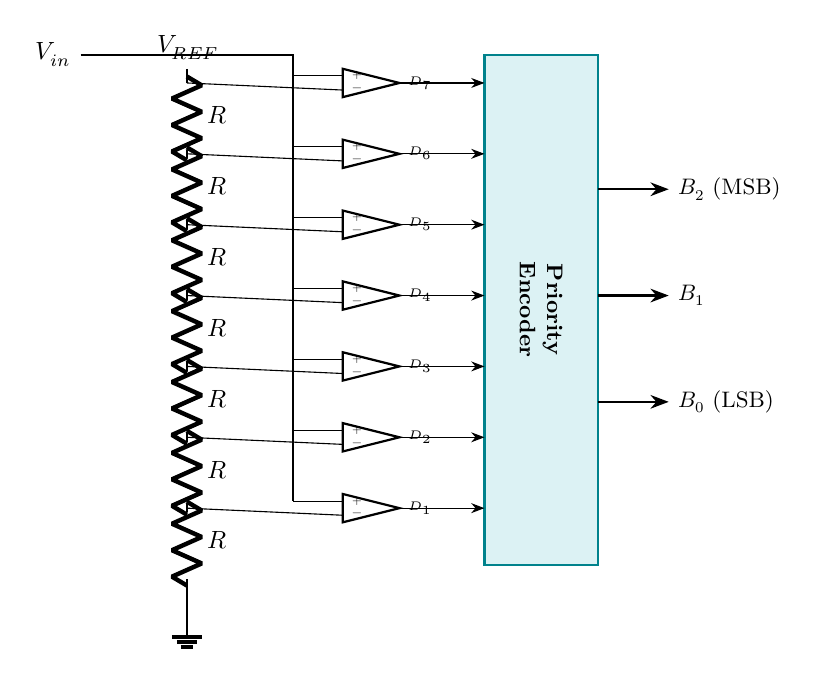
\begin{tikzpicture}[scale=0.9, transform shape]
  % Resistor ladder
  \draw[thick] (0, 3.2) node[above] {$V_{REF}$} -- (0, 3) to[R, l=$R$] (0, 2) to[R, l=$R$] (0, 1) to[R, l=$R$] (0, 0) to[R, l=$R$] (0, -1) to[R, l=$R$] (0, -2) to[R, l=$R$] (0, -3) to[R, l=$R$] (0, -4) -- (0, -4.4) node[ground] {};

  % Comparators
  \foreach \y/\i in {3/7, 2/6, 1/5, 0/4, -1/3, -2/2, -3/1} {
    \draw[thick] (2.2, \y-0.2) -- (2.2, \y+0.2) -- (3.0, \y) -- cycle;
    \node[font=\tiny] at (2.4, \y+0.1) {$+$};
    \node[font=\tiny] at (2.4, \y-0.1) {$-$};
    \node[right, font=\tiny] at (3.0, \y) {$D_{\i}$};
    
    % Connections
    \draw (0, \y) -- (2.2, \y-0.1); % connects to negative
  }

  % Common input line Vin
  \draw[thick] (-1.5, 3.4) node[left] {$V_{in}$} -- (1.5, 3.4) -- (1.5, -2.9);
  \foreach \y in {3, 2, 1, 0, -1, -2, -3} {
    \draw (1.5, \y+0.1) -- (2.2, \y+0.1); % connects to positive
  }

  % Encoder Block
  \draw[thick, fill=hdrteal, draw=myteal] (4.2, -3.8) rectangle (5.8, 3.4);
  \node[rotate=-90, font=\small\bfseries, align=center] at (5.0, -0.2) {Priority\\Encoder};
  
  % Connections from comparators to encoder
  \foreach \y in {3, 2, 1, 0, -1, -2, -3} {
    \draw[-Stealth] (3.0, \y) -- (4.2, \y);
  }

  % Outputs
  \draw[-Stealth, thick] (5.8, 1.5) -- (6.8, 1.5) node[right, font=\small] {$B_2$ (MSB)};
  \draw[-Stealth, thick] (5.8, 0.0) -- (6.8, 0.0) node[right, font=\small] {$B_1$};
  \draw[-Stealth, thick] (5.8, -1.5) -- (6.8, -1.5) node[right, font=\small] {$B_0$ (LSB)};
\end{tikzpicture}
\end{tcolorbox}

\begin{itemize}[leftmargin=*, itemsep=2pt]
  \item \textbf{Working:} The resistor ladder sets $2^N-1$ reference voltages. The comparators simultaneously compare $V_{in}$ to these references, producing a thermometer code. The priority encoder translates this thermometer code to an $N$-bit binary code.
  \item \textbf{Pros:} Conversion finishes in a single clock cycle (highest speed, GHz range).
  \item \textbf{Cons:} Component count grows exponentially ($2^N-1$ comparators). Power and input capacitance grow heavily, limiting resolution to 8 bits.
\end{itemize}

\subsection{2. Successive Approximation Register (SAR) ADC (Moderate Speed/Resolution)}
The SAR ADC utilizes a binary search algorithm to resolve the input voltage bit-by-bit over $N$ clock cycles.
\begin{itemize}[leftmargin=*, itemsep=2pt]
  \item \textbf{Working:} The Sample-and-Hold circuit holds $V_{in}$. The SAR logic sets the MSB of the DAC to 1. The comparator compares $V_{in}$ to $V_{DAC}$. If $V_{in} > V_{DAC}$, the MSB remains 1; otherwise, it is reset to 0. The process repeats for the next bit until all $N$ bits are resolved.
  \item \textbf{Pros:} Low power, minimal analog hardware (only 1 comparator, 1 DAC, and control logic).
  \item \textbf{Cons:} Requires $N$ clock cycles per conversion, limiting speed.
\end{itemize}

\subsection{3. Dual-Slope Integrator ADC (High Accuracy/Low Speed)}
A dual-slope ADC integrates the input voltage for a fixed time $T_1$, then de-integrates using a reference voltage $V_{REF}$ until the integrator output returns to zero.
\begin{itemize}[leftmargin=*, itemsep=2.5pt]
  \item \textbf{Working:} The integrator charges up with current $I_1 = V_{in}/R$ for $2^N$ clock cycles. Then, the input is switched to $-V_{REF}$, discharging the integrator back to 0. A counter measures the discharge time $T_2$.
  \item \textbf{Equation:} The peak integrator voltage is $V_p = \frac{V_{in}}{RC} T_1 = \frac{V_{REF}}{RC} T_2 \Rightarrow V_{in} = V_{REF} \frac{T_2}{T_1}$.
  \item \textbf{Pros:} Outstanding noise rejection (integrates thermal noise out). The accuracy is independent of clock frequency and component values ($R$ and $C$).
  \item \textbf{Cons:} Extremely slow ($2^{N+1}$ clock cycles per sample). Used in digital multimeters.
\end{itemize}

\subsection{4. Pipeline ADC (High Speed, Medium-High Resolution)}
A Pipeline ADC achieves high throughput by processing multiple samples concurrently across a chain of stages. Each stage resolves a coarse set of bits, computes the remaining error (residue), amplifies it by $\times 2$, and passes it to the next stage.

\begin{tcolorbox}[tikzbox, title={Pipeline ADC: 1.5-Bit Stage Architecture}]
\centering
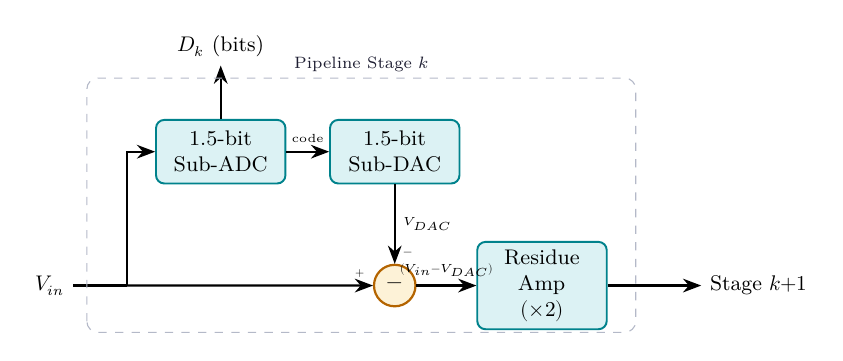
\begin{tikzpicture}[scale=0.85, transform shape]
  % Nodes
  \node[block, text width=1.7cm] (sadc) at (0, 1.2) {1.5-bit\\Sub-ADC};
  \node[block, text width=1.7cm] (sdac) at (2.6, 1.2) {1.5-bit\\Sub-DAC};
  \node[sumjunc] (sub) at (2.6, -0.8) {$-$};
  \node[block, text width=1.7cm] (amp) at (4.8, -0.8) {Residue Amp\\$(\times 2)$};

  % Inputs and Split
  \draw[thick] (-2.2, -0.8) node[left, font=\small]{$V_{in}$} -- (-1.4, -0.8);
  \draw[-Stealth, thick] (-1.4, -0.8) |- (sadc.west);
  \draw[-Stealth, thick] (-1.4, -0.8) -- (sub.west);
  
  \node[above left, font=\tiny] at (sub.west) {$+$};
  \node[above right, font=\tiny] at (sub.north) {$-$};

  % ADC to DAC
  \draw[-Stealth, thick] (sadc.east) -- (sdac.west) node[midway, above, font=\tiny]{code};

  % Digital output
  \draw[-Stealth, thick] (sadc.north) -- ++(0, 0.8) node[above, font=\small]{$D_k$ (bits)};

  % DAC to subtractor
  \draw[-Stealth, thick] (sdac.south) -- (sub.north) node[midway, right, font=\tiny]{$V_{DAC}$};

  % Subtractor to amp
  \draw[-Stealth, thick] (sub.east) -- (amp.west) node[midway, above, font=\tiny]{$(V_{in}{-}V_{DAC})$};

  % Output to next stage
  \draw[-Stealth, thick] (amp.east) -- ++(1.4, 0) node[right, font=\small]{Stage $k{+}1$};

  % Stage bounding box
  \draw[dashed, color=mgframe, rounded corners=4pt] (-2.0, -1.5) rectangle (6.2, 2.3);
  \node[font=\scriptsize\color{mydark}] at (2.1, 2.5) {Pipeline Stage $k$};
\end{tikzpicture}
\end{tcolorbox}

\textbf{Working (1.5-bit/stage):}
\begin{enumerate}[label=\textbf{\arabic*.}, leftmargin=*, itemsep=3pt]
  \item \textbf{Sub-ADC:} A 2-comparator flash resolves the MSBs using three levels ($+1$, $0$, $-1$) compared against $\pm V_{REF}/4$.
  \item \textbf{Sub-DAC:} The coarse code is converted back to an analog level $V_{DAC}$.
  \item \textbf{Residue Amplifier (MDAC):} Computes $V_{res} = 2(V_{in} - V_{DAC})$, scaling the residue to fill the full input range of the next stage.
  \item \textbf{Pipelining:} While Stage 1 processes sample $n+1$, Stage 2 concurrently processes the residue of sample $n$. This gives one output code per clock cycle after an initial latency of $N_{stages}$ cycles.
  \item \textbf{Digital Error Correction:} The 0.5-bit redundancy allows the back-end logic to correct comparator offset errors up to $\pm V_{REF}/4$, relaxing hardware specifications significantly.
\end{enumerate}
\begin{itemize}[leftmargin=*, itemsep=2pt]
  \item \textbf{Pros:} High throughput (10\,Msps--1\,Gsps), excellent resolution (10--14 bits).
  \item \textbf{Cons:} Multi-cycle pipeline latency; MDAC gain accuracy critically limits INL.
\end{itemize}

\subsection{5. Hybrid ADC Structures}
Hybrid ADCs merge two architectures to combine the speed strength of one with the resolution or power efficiency of the other.

\begin{tcolorbox}[defbox, title={\textbf{Common Hybrid ADC Topologies}}]
\begin{itemize}[leftmargin=*, itemsep=4pt, topsep=0pt]
  \item \textbf{Flash-SAR Hybrid:} A coarse Flash ADC resolves the top $M$ bits in a single cycle; a SAR ADC then refines the residue over $N{-}M$ cycles. Reduces comparator count from $2^N - 1$ (full Flash) to $2^M + N - M$, saving power while maintaining near-Flash speed.
  \item \textbf{Pipelined-SAR (SAR-assisted Pipeline):} Each pipeline stage employs a short SAR loop (4--6 bits) instead of the traditional 1.5-bit MDAC. This reduces the total number of stages and relaxes the MDAC gain-bandwidth requirement. Dominant in 10--14-bit, 50--500\,Msps ADCs in modern scaled CMOS nodes.
  \item \textbf{Incremental $\Delta\Sigma$ ADC:} Resets its accumulator after each conversion cycle, combining $\Delta\Sigma$ noise-shaping with discrete Nyquist-rate output. Used in precision multi-channel sensor readout (industrial, medical, weighing systems).
\end{itemize}
\end{tcolorbox}

\subsection{6. Delta-Sigma (\texorpdfstring{$\Delta\Sigma$}{Delta-Sigma}) ADC (Oversampling \& Noise Shaping)}
Delta-Sigma ADCs achieve ultra-high resolution ($16\text{--}24$ bits) by combining \textbf{Oversampling} and \textbf{Noise Shaping}.

\begin{tcolorbox}[tikzbox, title={First-Order Delta-Sigma Modulator Block Diagram}]
\centering
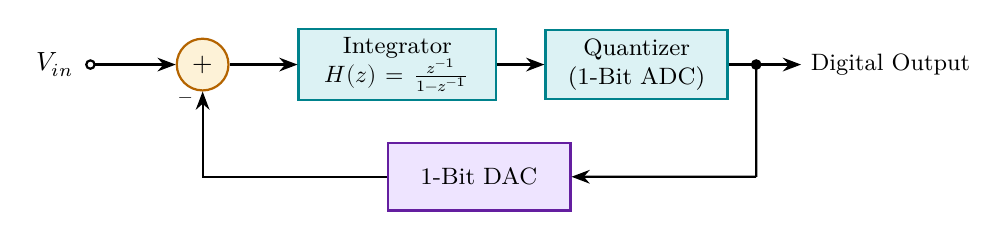
\begin{tikzpicture}[scale=0.95, transform shape]
  % Input
  \node[left] at (-1.6, 0) {$V_{in}$};
  
  % Summer
  \node[draw=myamber, fill=hdramber, circle, minimum size=0.6cm, thick] (sum) at (0, 0) {$+$};
  \draw[-Stealth, thick] (-1.5, 0) to[short, o-] (sum.west);
  
  % Integrator
  \node[draw=myteal, fill=hdrteal, minimum width=1.5cm, minimum height=0.9cm, font=\small, thick, align=center, text width=2.4cm] (int) at (2.6, 0) {Integrator\\$H(z) = \frac{z^{-1}}{1-z^{-1}}$};
  \draw[-Stealth, thick] (sum) -- (int);
  
  % Quantizer (ADC)
  \node[draw=myteal, fill=hdrteal, minimum width=1.4cm, minimum height=0.9cm, font=\small, thick, align=center, text width=2.2cm] (quant) at (5.8, 0) {Quantizer\\(1-Bit ADC)};
  \draw[-Stealth, thick] (int) -- (quant);
  
  % Output
  \draw[-Stealth, thick] (quant) -- (8.0, 0) node[right, font=\small] {Digital Output};
  \draw[thick] (7.4, 0) to[short, *-] (7.4, -1.5);
  
  % Feedback DAC
  \node[draw=mypurple, fill=hdrpurple, minimum width=1.4cm, minimum height=0.9cm, font=\small, thick, align=center, text width=2.2cm] (dac) at (3.7, -1.5) {1-Bit DAC};
  \draw[-Stealth, thick] (7.4, -1.5) -- (dac);
  \draw[-Stealth, thick] (dac) -| (sum) node[left, pos=0.95, font=\scriptsize] {$-$};
\end{tikzpicture}
\end{tcolorbox}

\textbf{Oversampling:} The input is sampled at $f_s \gg 2f_{max}$. The Oversampling Ratio is $\text{OSR} = f_s / (2 f_{max})$. Oversampling spreads the same quantization noise power $\Delta^2/12$ over a wider bandwidth $f_s/2$, reducing the noise spectral density in the signal band.

\textbf{Noise Shaping:} By placing the quantizer inside a feedback loop with an integrator, the transfer function shapes the quantization noise. The output in the Z-domain is:
\[
Y(z) = X(z) z^{-1} + E(z)(1 - z^{-1})
\]
This shows that the input signal $X(z)$ is passed with a simple delay (Signal Transfer Function $\text{STF}(z) = z^{-1}$), while the quantization noise $E(z)$ is high-pass filtered (Noise Transfer Function $\text{NTF}(z) = 1-z^{-1}$). The noise is pushed out of the low-frequency signal band into high frequencies, where it is easily removed by a digital decimation filter.

% ===============================================================================
\section{Digital-to-Analog Converter (DAC) Architectures}
% ===============================================================================

\subsection{1. R-2R Ladder DAC (Compact Layout)}
Unlike binary-weighted resistor DACs (which require huge component ratios like $2^N:1$), the R-2R ladder uses only two resistor values ($R$ and $2R$), making matching very easy.

The output voltage is:
\[
V_{out} = V_{REF} \sum_{i=1}^{N} \frac{b_i}{2^i}
\]
where $b_1$ is the MSB and $b_N$ is the LSB.

\subsection{2. Current-Steering DAC (High Speed)}
Current-steering DACs route currents from matched MOS current sources to the output node based on the digital input code.
\begin{itemize}[leftmargin=*, itemsep=2pt]
  \item \textbf{Working:} An array of current sources (either binary-weighted or thermometer-coded) is connected to differential switches. Thermometer coding is preferred for high resolution because it guarantees monotonicity and minimizes output glitches, though it requires a thermometer decoder.
  \item \textbf{Pros:} Extremely fast (up to GHz range), can drive resistive loads (like $50\,\Omega$ coaxial cables) directly.
\end{itemize}

% ===============================================================================
% QUICK REVISION PAGE
% ===============================================================================
\newpage
\begin{center}
  {\large\bfseries\color{myred} Quick Revision --- Module 3}\\[3pt]
  {\small\color{mydark} Data Converters $|$ PE-EC802A}
\end{center}
\noindent{\color{myred}\rule{\linewidth}{1.2pt}}
\vspace{4pt}

\begin{tcolorbox}[formulabox, title={\textbf{Key Formulas at a Glance}}]
\renewcommand{\arraystretch}{1.35}
\begin{tabularx}{\linewidth}{B{5.0cm} X}
Quantization Error Power & $P_{qn} = \frac{\Delta^2}{12}$ \\[4pt]
Ideal SQNR (dB) & $\text{SQNR} = 6.02 N + 1.76\,$dB \\[4pt]
Oversampling Ratio (OSR) & $\text{OSR} = \frac{f_s}{2 f_{max}}$ \\[4pt]
1st-Order Modulator NTF & $\text{NTF}(z) = 1 - z^{-1}$ \\[4pt]
2nd-Order Modulator NTF & $\text{NTF}(z) = (1 - z^{-1})^2$ \\[4pt]
Flash Comparator Count & $N_{comp} = 2^N - 1$ \\[4pt]
Dual-Slope conversion time & $T_{conv} \approx 2^{N+1} T_{clk}$ \\
\end{tabularx}
\end{tcolorbox}

\begin{tcolorbox}[defbox, title={\textbf{One-Line Definitions}}]
\begin{itemize}[leftmargin=*, itemsep=2pt, topsep=0pt]
  \item \textbf{DNL:} The deviation of an actual step size from the ideal $1\,\text{LSB}$ step width.
  \item \textbf{INL:} The cumulative deviation of the actual transfer curve from the ideal straight line.
  \item \textbf{Oversampling:} Sampling a signal at a rate significantly higher than the Nyquist rate.
  \item \textbf{Noise Shaping:} Pushing quantization noise from the signal band to higher frequencies using feedback loops.
  \item \textbf{Monotonicity:} A converter characteristic where the output always increases or stays constant as input increases.
  \item \textbf{Thermometer Code:} A unary code format representing value $K$ by $K$ consecutive ones (e.g., $3 \rightarrow 0000111$).
  \item \textbf{Missing Codes:} An ADC defect where certain output codes are skipped, caused by $\text{DNL} < -1\,\text{LSB}$.
  \item \textbf{Pipeline ADC:} A high-speed converter using chained 1.5-bit stages with residue amplification, enabling one output per clock cycle.
  \item \textbf{Hybrid ADC:} A converter combining two architectures (e.g., Flash-SAR, Pipelined-SAR) to trade off speed, resolution, and power.
\end{itemize}
\end{tcolorbox}

\begin{tcolorbox}[tikzbox, title={\textbf{ADC Architecture Comparison at a Glance}}]
\centering
\par\noindent
\renewcommand{\arraystretch}{1.25}
\begin{tabularx}{\linewidth}{|B{2.2cm}|Y|Y|Y|Y|}
\hline
\textbf{ADC Type} & \textbf{Speed} & \textbf{Resolution} & \textbf{Power} & \textbf{Application} \\ \hline
\textbf{Flash} & GHz range & $\leq$8 bit & Very High & Oscilloscopes, SerDes \\ \hline
\textbf{SAR} & $<$100\,Msps & 8--18 bit & Very Low & Sensors, IoT, MCUs \\ \hline
\textbf{Dual-Slope} & $<$100 sps & 20+ bit & Low & Multimeters \\ \hline
\textbf{Pipeline} & 10--1000\,Msps & 10--14 bit & Medium & WLAN, Video, RADAR \\ \hline
\textbf{$\Delta\Sigma$} & $<$10\,Msps & 16--24 bit & Medium & Audio, Precision \\ \hline
\textbf{Hybrid} & Varies & Varies & Low--Medium & Imaging, Comm. IC \\ \hline
\end{tabularx}
\end{tcolorbox}

\begin{tcolorbox}[exambox, title={\textbf{Frequently Asked / Viva Questions}}]
\begin{enumerate}[topsep=0pt, label=\textbf{Q\arabic*.}, itemsep=5pt]
  \item \Q{Derive the quantization noise power of an ideal ADC.}
    For a quantization step size $\Delta$, the error $e$ is uniformly distributed between $-\Delta/2$ and $\Delta/2$ with PDF $1/\Delta$. The noise power is the variance: $P_{qn} = \int_{-\Delta/2}^{\Delta/2} e^2 (1/\Delta) de = [e^3/3\Delta]_{-\Delta/2}^{\Delta/2} = \Delta^2/12$.
  \item \Q{What causes missing codes in an ADC, and how is it defined mathematically?}
    Missing codes occur when the transition step width of a digital code is zero or negative. This happens when the Differential Non-Linearity (DNL) at that code is less than or equal to $-1\,\text{LSB}$.
  \item \Q{Explain the trade-offs of Flash ADC architecture.}
    Flash ADC is the fastest architecture because it performs parallel comparisons in one clock cycle. However, it requires $2^N - 1$ comparators. This causes exponential growth in area, power dissipation, and input capacitance, limiting the resolution to 8 bits.
  \item \Q{How does a Delta-Sigma ADC achieve very high resolution?}
    By combining oversampling (which spreads quantization noise over a wider band) and noise shaping (which uses a loop filter to push noise to high frequencies). A digital low-pass decimation filter then filters out the out-of-band noise, leaving a high-resolution signal.
  \item \Q{Why is a dual-slope ADC highly accurate, and where is it used?}
    Its accuracy depends only on the ratio of charging and discharging times ($T_2/T_1$), which is independent of the absolute values of $R$, $C$, and clock frequency. It is used in digital multimeters where accuracy is critical and speed is not.
  \item \Q{Compare SAR and Flash ADCs in terms of speed, area, and power.}
    Flash ADC converts in 1 clock cycle but requires $2^N-1$ comparators (huge area and power). SAR ADC takes $N$ clock cycles but requires only 1 comparator and 1 DAC, resulting in very low power and compact area.
  \item \Q{What is the benefit of the R-2R ladder DAC over a binary-weighted resistor DAC?}
    A binary-weighted resistor DAC requires a very wide range of resistor values ($2^N:1$), which is difficult to match on-chip. The R-2R ladder DAC uses only two resistor values ($R$ and $2R$), ensuring excellent matching and layout compacting.
  \item \Q{Explain the function of the priority encoder in a Flash ADC.}
    The comparators output a thermometer code (e.g. 0000111). The priority encoder identifies the highest active input line and converts that thermometer code into standard binary output (e.g. 011).
  \item \Q{What is the Noise Transfer Function (NTF) of a first-order Delta-Sigma modulator?}
    The NTF is a high-pass filter: $\text{NTF}(z) = 1 - z^{-1}$. In the frequency domain, it is $2 \sin(\omega T_s /2)$, which attenuates noise near DC and amplifies it at high frequencies.
  \item \Q{What is the difference between DNL and INL?}
    DNL is the local step size error from the ideal $1\,\text{LSB}$ step width. INL is the global deviation of the actual transfer function from the ideal straight line, equal to the cumulative sum of the DNL errors.
\end{enumerate}
\end{tcolorbox}


% -- Module 4 -----------------------------------------------------------------
\modulestart{4}{Mixed-Signal Layout Issues \& Mitigation}

\section{Mixed-Signal Layout Issues \& Mitigation}
% ===============================================================================

In high-performance mixed-signal integrated circuits, fast-switching digital gates inject noise into the shared silicon substrate and power distribution networks, which severely degrades the resolution of sensitive analog blocks (like ADCs and low-noise amplifiers).

\subsection{1. Substrate Coupling}
Digital circuits consist of logic gates that switch states rapidly, drawing transient currents from the supplies. When the source/drain terminals of digital transistors transition, charge is coupled into the common p-substrate wafer via junction capacitances. This noise propagates through the conductive substrate to sensitive analog devices.

\begin{tcolorbox}[tikzbox, title={Cross-Sectional Model of Substrate Noise Coupling and Guard Ring Protection}]
\centering
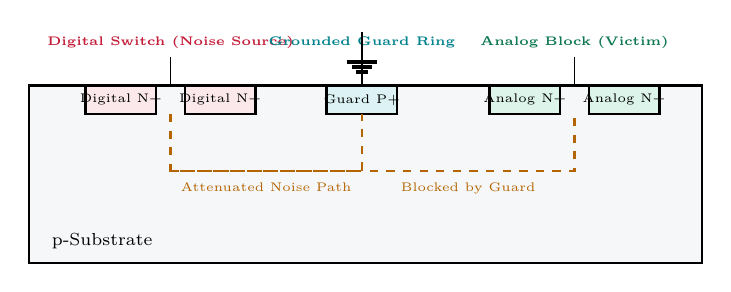
\begin{tikzpicture}[scale=0.9, transform shape]
  % Wafer substrate
  \draw[thick, fill=mygray] (0, 0) rectangle (9.5, -2.5);
  \node[right, font=\scriptsize] at (0.2, -2.2) {p-Substrate};
  
  % Digital noise source (N+ regions)
  \draw[thick, fill=hdrred] (0.8, 0) rectangle (1.8, -0.4);
  \node[font=\tiny] at (1.3, -0.2) {Digital N+};
  \draw[thick, fill=hdrred] (2.2, 0) rectangle (3.2, -0.4);
  \node[font=\tiny] at (2.7, -0.2) {Digital N+};
  \node[above, font=\tiny\bfseries\color{myred}] at (2.0, 0.4) {Digital Switch (Noise Source)};
  \draw (2.0, 0.4) -- (2.0, 0);

  % Guard Ring (P+ region)
  \draw[thick, fill=hdrteal] (4.2, 0) rectangle (5.2, -0.4);
  \node[font=\tiny] at (4.7, -0.2) {Guard P+};
  \node[above, font=\tiny\bfseries\color{myteal}] at (4.7, 0.4) {Grounded Guard Ring};
  \draw[thick] (4.7, 0) -- (4.7, 0.75) node[ground] {};

  % Analog noise victim (N+ regions)
  \draw[thick, fill=hdrgreen] (6.5, 0) rectangle (7.5, -0.4);
  \node[font=\tiny] at (7.0, -0.2) {Analog N+};
  \draw[thick, fill=hdrgreen] (7.9, 0) rectangle (8.9, -0.4);
  \node[font=\tiny] at (8.4, -0.2) {Analog N+};
  \node[above, font=\tiny\bfseries\color{mygreen}] at (7.7, 0.4) {Analog Block (Victim)};
  \draw (7.7, 0.4) -- (7.7, 0);

  % Substrate resistance network (noise paths)
  \draw[thick, dashed, color=myamber] (2.0, -0.4) -- (2.0, -1.2) -- (4.7, -1.2);
  \draw[thick, dashed, color=myamber] (4.7, -1.2) -- (4.7, -0.4);
  \draw[thick, dashed, color=myamber] (2.0, -1.2) -- (7.7, -1.2) -- (7.7, -0.4);
  
  \node[below, font=\tiny\color{myamber}] at (3.35, -1.25) {Attenuated Noise Path};
  \node[below, font=\tiny\color{myamber}] at (6.2, -1.25) {Blocked by Guard};
\end{tikzpicture}
\end{tcolorbox}

\textbf{Mitigation Strategy (Guard Rings):}
A guard ring is a low-impedance ring of diffusion surrounding the circuit blocks.
\begin{itemize}[leftmargin=*, itemsep=2.5pt]
  \item \textbf{p+ Guard Ring:} Implemented in p-substrate, connected to a dedicated quiet analog ground ($V_{SSA}$). It collects hole currents flowing through the substrate from digital noise sources, shunting them to ground before they reach the analog block.
  \item \textbf{n+ Guard Ring in N-well:} Connected to quiet supply ($V_{DDA}$), collecting electron currents and isolating regions.
\end{itemize}

\subsection{2. Power Supply Noise and Ground Bounce}
Power and ground pads on an IC package exhibit parasitic inductance ($L$) and resistance ($R$). When digital gates switch simultaneously, they draw sharp current spikes ($di/dt$), causing a voltage fluctuation on the supply rails:
\[
V_{bounce} = L \frac{di}{dt}
\]
This fluctuation directly modulates the threshold voltages and bias conditions of analog circuits connected to the same supply rails.

\textbf{Mitigation:}
\begin{itemize}[leftmargin=*, itemsep=2pt]
  \item \textbf{Split Supplies:} Separate supply pins and routing traces for analog ($V_{DDA}, V_{SSA}$) and digital ($V_{DDD}, V_{SSD}$) domains.
  \item \textbf{On-Chip Decoupling Capacitors (Decaps):} Placed near supply rails to act as local charge reservoirs, damping high-frequency voltage ripples.
\end{itemize}

\subsection{3. Interconnect Parasitics \& Signal Integrity}
At high frequencies, on-chip and on-board wires cannot be treated as ideal conductors. They exhibit distributed resistance ($r$), inductance ($l$), and capacitance ($c$) per unit length.

\begin{tcolorbox}[defbox, title={\textbf{Interconnect Lumped RLC Model}}]
\begin{itemize}[leftmargin=*, itemsep=2pt, topsep=0pt]
  \item \textbf{Resistance $r$ ($\Omega$/m):} From metal sheet resistance. Causes $I^2R$ voltage drop and thermal loss.
  \item \textbf{Capacitance $c$ (F/m):} From metal-to-substrate or metal-to-metal coupling. Acts as a low-pass filter, limiting signal bandwidth: $f_{-3\text{dB}} \approx 1/(2\pi r c \ell^2)$.
  \item \textbf{Inductance $l$ (H/m):} Dominant at RF frequencies. Causes inductive ringing and reflections at impedance discontinuities.
\end{itemize}
\end{tcolorbox}

\textbf{Key Signal Integrity Issues:}
\begin{itemize}[leftmargin=*, itemsep=2.5pt]
  \item \textbf{Crosstalk:} Capacitive/inductive coupling between adjacent wires adds interference. Mitigated by inserting grounded shield traces between signal lines.
  \item \textbf{Reflections:} When a signal reaches an impedance discontinuity ($Z_L \neq Z_0$), part is reflected with coefficient:
  \[\Gamma = \frac{Z_L - Z_0}{Z_L + Z_0}\]
  Mitigated by matched termination ($Z_L = Z_0$, e.g., $50\,\Omega$ for coaxial cables).
  \item \textbf{Propagation Delay:} Signal propagation velocity is $v_p = 1/\sqrt{lc} \approx c_0/\sqrt{\varepsilon_r}$. For FR4 PCB ($\varepsilon_r \approx 4$): $v_p \approx 1.5 \times 10^8\,$m/s.
\end{itemize}

% ===============================================================================
\section{Device Matching and Precision Layout}
% ===============================================================================

Matching of on-chip components (capacitors and transistors) is critical for accuracy in data converters and differential amplifiers.

\subsection{1. Types of Mismatch}
Mismatch is categorized as systematic or random.
\begin{itemize}[leftmargin=*, itemsep=2.5pt]
  \item \textbf{Systematic Mismatch:} Caused by deterministic spatial gradients across the wafer (e.g., temperature variations, oxide thickness gradients, lithography light scattering).
  \item \textbf{Random Mismatch:} Caused by microscopic statistical variations (e.g., edge roughness, dopant atom fluctuations).
\end{itemize}

\subsection{2. Common-Centroid Matching for Capacitors}
To cancel the effects of linear spatial gradients (such as oxide thickness variations across a wafer), matching devices must be arranged symmetrically about a common central point (common-centroid configuration).

Consider matching two equal capacitors $C_A$ and $C_B$. If they are placed side-by-side ($A$ next to $B$), a linear gradient in oxide thickness will cause one to be larger than the other. If we split each capacitor into two halves ($A_1, A_2$ and $B_1, B_2$) and arrange them in a one-dimensional or two-dimensional array, the gradient effects cancel.

\begin{tcolorbox}[tikzbox, title={Common-Centroid Capacitor Array Layout (ABBA)}]
\centering
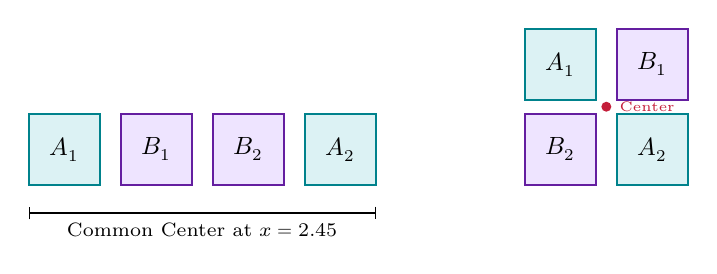
\begin{tikzpicture}[scale=0.9]
  % 1D Common Centroid: A B B A
  \draw[thick, fill=hdrteal, draw=myteal] (0,0) rectangle (1,1) node[pos=0.5, font=\small\bfseries] {$A_1$};
  \draw[thick, fill=hdrpurple, draw=mypurple] (1.3,0) rectangle (2.3,1) node[pos=0.5, font=\small\bfseries] {$B_1$};
  \draw[thick, fill=hdrpurple, draw=mypurple] (2.6,0) rectangle (3.6,1) node[pos=0.5, font=\small\bfseries] {$B_2$};
  \draw[thick, fill=hdrteal, draw=myteal] (3.9,0) rectangle (4.9,1) node[pos=0.5, font=\small\bfseries] {$A_2$};
  
  \draw[|-|] (0,-0.4) -- (4.9,-0.4) node[midway, below, font=\scriptsize] {Common Center at $x = 2.45$};
  
  % 2D Common Centroid Box: 
  % A B
  % B A
  \begin{scope}[xshift=7cm]
    \draw[thick, fill=hdrteal, draw=myteal] (0,1.2) rectangle (1,2.2) node[pos=0.5, font=\small\bfseries] {$A_1$};
    \draw[thick, fill=hdrpurple, draw=mypurple] (1.3,1.2) rectangle (2.3,2.2) node[pos=0.5, font=\small\bfseries] {$B_1$};
    \draw[thick, fill=hdrpurple, draw=mypurple] (0,0) rectangle (1,1) node[pos=0.5, font=\small\bfseries] {$B_2$};
    \draw[thick, fill=hdrteal, draw=myteal] (1.3,0) rectangle (2.3,1) node[pos=0.5, font=\small\bfseries] {$A_2$};
    
    \fill[myred] (1.15, 1.1) circle (2pt);
    \node[right, font=\tiny\color{myred}] at (1.2, 1.1) {Center};
  \end{scope}
\end{tikzpicture}
\end{tcolorbox}

By connecting $A = A_1 + A_2$ and $B = B_1 + B_2$, any linear variation in the horizontal or vertical direction affects both groups equally, preserving the ratio $C_A/C_B = 1$.

% ===============================================================================
\section{Low-Voltage Differential Signaling (LVDS)}
% ===============================================================================

\subsection{Single-Ended vs. Differential Signaling}
Single-ended signaling routes signals as a voltage relative to a common ground rail. Any ground bounce or external electromagnetic coupling adds directly to the signal, corrupting it.

Differential signaling uses two complementary lines ($V_p$ and $V_n$) to transmit information. The receiver detects only the difference $V_{diff} = V_p - V_n$.
\begin{itemize}[leftmargin=*, itemsep=2.5pt]
  \item \textbf{Common-Mode Rejection:} Any noise coupled onto the board affects both lines equally. Since the receiver processes only the difference, this common-mode noise is rejected.
  \item \textbf{Reduced EMI:} The magnetic fields generated by the current in the two tightly-coupled differential traces are equal and opposite, cancelling out, which minimizes electromagnetic interference (EMI).
\end{itemize}

\subsection{LVDS Transceiver Interface}
LVDS is a high-speed, low-power physical layer interface standard. It operates by routing a constant current through a differential pair terminated by a resistor.

\begin{tcolorbox}[tikzbox, title={LVDS Transceiver Interface Schematic}]
\centering
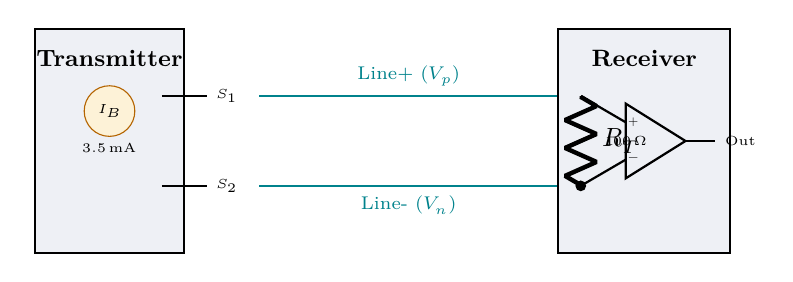
\begin{tikzpicture}[scale=0.95, transform shape]
  % Transmitter box
  \draw[thick, fill=hdrgray] (-2.5, 1.5) rectangle (-0.5, -1.5);
  \node[font=\small\bfseries] at (-1.5, 1.1) {Transmitter};
  \node[draw=myamber, fill=hdramber, circle, minimum size=0.5cm, font=\tiny] (ib) at (-1.5, 0.4) {$I_B$};
  \node[below, font=\tiny] at (-1.5, 0.1) {$3.5\,$mA};
  
  % Switches
  \draw[thick] (-0.8, 0.6) -- (-0.2, 0.6) node[right, font=\tiny] {$S_1$};
  \draw[thick] (-0.8, -0.6) -- (-0.2, -0.6) node[right, font=\tiny] {$S_2$};
  
  % Transmission Lines
  \draw[thick, color=myteal] (0.5, 0.6) -- (4.5, 0.6) node[midway, above, font=\scriptsize] {Line+ ($V_p$)};
  \draw[thick, color=myteal] (0.5, -0.6) -- (4.5, -0.6) node[midway, below, font=\scriptsize] {Line- ($V_n$)};
  
  % Receiver
  \draw[thick, fill=hdrgray] (4.5, 1.5) rectangle (6.8, -1.5);
  \node[font=\small\bfseries] at (5.65, 1.1) {Receiver};
  
  % Termination resistor
  \draw[thick] (4.8, 0.6) to[R, l=$R_T$, -*] (4.8, -0.6);
  \node[right, font=\tiny] at (5.0, 0.0) {$100\,\Omega$};
  
  % Differential Receiver Op-amp
  \draw[thick] (5.4, 0.5) -- (5.4, -0.5) -- (6.2, 0.0) -- cycle;
  \node[font=\tiny] at (5.5, 0.25) {$+$};
  \node[font=\tiny] at (5.5, -0.25) {$-$};
  \draw[thick] (4.8, 0.6) -- (5.4, 0.25);
  \draw[thick] (4.8, -0.6) -- (5.4, -0.25);
  \draw[thick] (6.2, 0.0) -- (6.6, 0.0) node[right, font=\tiny] {Out};
\end{tikzpicture}
\end{tcolorbox}

\textbf{Key Parameters:}
\begin{enumerate}[label=\textbf{\arabic*.}, leftmargin=*, itemsep=3.5pt]
  \item \textbf{Current Loop:} The transmitter contains a $3.5\,$mA current source. Depending on the digital state, the switches route this current down either $V_p$ or $V_n$.
  \item \textbf{Termination:} The current flows through the transmission line and passes through the $100\,\Omega$ termination resistor $R_T$ at the receiver, then returns via the other line.
  \item \textbf{Voltage Swing:} The voltage swing across $R_T$ is:
  \[
  V_{diff} = I_{loop} \times R_T = 3.5\,\text{mA} \times 100\,\Omega = 350\,\text{mV}
  \]
  This small voltage swing allows extremely fast switching and minimizes power consumption.
  \item \textbf{Common-Mode Voltage:} The nominal common-mode voltage is set to $1.2\,$V, which is compatible with low-voltage supply rails.
\end{enumerate}

% ===============================================================================
\section{Current-Mode Logic (CML) Signaling}
% ===============================================================================

\begin{tcolorbox}[defbox, title={\textbf{Current-Mode Logic (CML) Concept}}]
\textbf{Current-Mode Logic (CML)} routes a constant tail current $I_{SS}$ through a differential transistor pair. The input data steers the current between two complementary output branches. Since the total current is always constant, the power rails see no transient spikes, and switching speed is limited only by the transistor $f_T$ and the load $R_L C_{load}$ time constant --- enabling multi-gigabit ($>$10\,Gbps) signaling.
\end{tcolorbox}

\begin{tcolorbox}[tikzbox, title={CML Differential Pair Gate Schematic}]
\centering
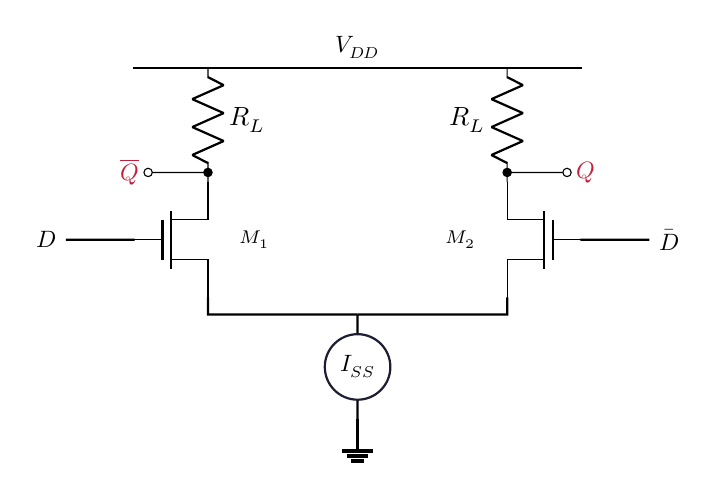
\begin{tikzpicture}[scale=0.95, transform shape]
  % VDD rail
  \draw[thick] (0.5, 3.8) -- (6.5, 3.8);
  \node[above, font=\small] at (3.5, 3.8) {$V_{DD}$};

  % Left load R_L
  \draw (1.5, 3.8) to[R, l=$R_L$] (1.5, 2.4);

  % Right load R_L
  \draw (5.5, 3.8) to[R, l_=$R_L$] (5.5, 2.4);

  % Transistors
  \node[nmos] (M1) at (1.5, 1.5) {};
  \node[nmos, xscale=-1] (M2) at (5.5, 1.5) {};
  
  \node[right, font=\scriptsize] at (1.8, 1.5) {$M_1$};
  \node[left, font=\scriptsize] at (5.2, 1.5) {$M_2$};

  % Connections to D and D_bar
  \draw[thick] (M1.gate) -- (-0.4, 1.5) node[left, font=\small] {$D$};
  \draw[thick] (M2.gate) -- (7.4, 1.5) node[right, font=\small] {$\bar{D}$};

  % Output terminals Q and Q_bar
  \draw (1.5, 2.4) -- (M1.drain);
  \draw (5.5, 2.4) -- (M2.drain);
  
  \draw (1.5, 2.4) to[short, *-o] (0.7, 2.4) node[left, font=\small\color{myred}] {$\overline{Q}$};
  \draw (5.5, 2.4) to[short, *-o] (6.3, 2.4) node[right, font=\small\color{myred}] {$Q$};

  % Sources connected to tail current
  \draw[thick] (M1.source) -- (1.5, 0.5) -- (3.5, 0.5);
  \draw[thick] (M2.source) -- (5.5, 0.5) -- (3.5, 0.5);
  
  \node[draw=mydark, circle, minimum size=0.7cm, thick, font=\small] (iss) at (3.5, -0.2) {$I_{SS}$};
  \draw[thick] (3.5, 0.5) -- (iss);
  \draw[thick] (iss) -- (3.5, -0.9) node[ground] {};
\end{tikzpicture}
\end{tcolorbox}

\textbf{Key CML Equations:}
\begin{enumerate}[label=\textbf{\arabic*.}, leftmargin=*, itemsep=3.5pt]
  \item \textbf{Output Swing:} The differential voltage is set by the tail current and load resistance:
  \begin{tcolorbox}[formulabox, title={\textbf{CML Output Swing and Bandwidth}}]
  \[
  \Delta V_{out} = I_{SS} \times R_L \qquad \text{(Typical: } 200\,\text{mV} - 800\,\text{mV)}
  \]
  \[
  f_{-3\text{dB}} = \frac{1}{2\pi\, R_L\, C_{load}} \qquad \text{(bandwidth set by RC time constant)}
  \]
  \end{tcolorbox}
  \item \textbf{Constant Current:} $P = V_{DD} \times I_{SS}$ is independent of switching activity --- no transient supply spikes, making CML ideal for mixed-signal environments.
  \item \textbf{Common-Mode Level:} The output common mode is biased by the load: $V_{CM} = V_{DD} - I_{SS} R_L / 2$, allowing direct DC cascading of multiple CML stages.
\end{enumerate}
\begin{itemize}[leftmargin=*, itemsep=2pt]
  \item \textbf{Applications:} SerDes transceivers, high-speed clock distribution, PCIe/Ethernet physical layers, multi-gigabit backplanes.
\end{itemize}

% ===============================================================================
% QUICK REVISION PAGE
% ===============================================================================
\newpage
\begin{center}
  {\large\bfseries\color{myred} Quick Revision --- Module 4}\\[3pt]
  {\small\color{mydark} Layout \& Signaling $|$ PE-EC802A}
\end{center}
\noindent{\color{myred}\rule{\linewidth}{1.2pt}}
\vspace{4pt}

\begin{tcolorbox}[formulabox, title={\textbf{Key Formulas at a Glance}}]
\renewcommand{\arraystretch}{1.35}
\begin{tabularx}{\linewidth}{B{5.0cm} X}
Ground Bounce Voltage & $V_{bounce} = L \frac{di}{dt}$ \\[4pt]
LVDS Current Loop & $I_{loop} = 3.5\,$mA \\[4pt]
LVDS Differential Swing & $V_{diff} = I_{loop} \times R_T = 350\,$mV \\[4pt]
LVDS Termination Resistor & $R_T = 100\,\Omega$ \\[4pt]
LVDS Common-Mode Voltage & $V_{CM} = 1.2\,$V \\[4pt]
\end{tabularx}
\end{tcolorbox}

\begin{tcolorbox}[defbox, title={\textbf{One-Line Definitions}}]
\begin{itemize}[leftmargin=*, itemsep=2pt, topsep=0pt]
  \item \textbf{Substrate Coupling:} Injection of digital switching noise into the shared silicon substrate, victimizing analog nodes.
  \item \textbf{Guard Ring:} A low-resistance diffusion ring surrounding sensitive analog components to collect substrate noise currents.
  \item \textbf{Ground Bounce:} Inductive supply noise caused by high $di/dt$ transitions across package lead inductances.
  \item \textbf{Systematic Mismatch:} Mismatch on silicon caused by deterministic spatial gradients across the wafer.
  \item \textbf{Random Mismatch:} Mismatch on silicon caused by microscopic statistical variations (e.g., dopant fluctuations).
  \item \textbf{Common-Centroid Layout:} Symmetrical layout arrangement of matched devices around a single central point to cancel linear gradients.
  \item \textbf{LVDS:} A high-speed differential signaling standard transmitting data using a $3.5\,$mA current loop over a $100\,\Omega$ termination.
  \item \textbf{CML:} Current-Mode Logic --- routes a constant tail current $I_{SS}$ through a differential pair for multi-gigabit signaling.
  \item \textbf{Interconnect Parasitics:} Distributed R, L, C of on-chip/board wires causing RC delay, reflections, and crosstalk.
  \item \textbf{Reflection Coefficient:} $\Gamma = (Z_L - Z_0)/(Z_L + Z_0)$; zero for matched termination ($Z_L = Z_0$).
\end{itemize}
\end{tcolorbox}

\begin{tcolorbox}[tikzbox, title={\textbf{High-Speed Signaling Interface Comparison}}]
\centering
\par\noindent
\renewcommand{\arraystretch}{1.3}
\begin{tabularx}{\linewidth}{|B{2.4cm}|Y|Y|Y|}
\hline
\textbf{Parameter} & \textbf{CMOS (Single-Ended)} & \textbf{LVDS} & \textbf{CML} \\ \hline
\textbf{Signal Swing} & $V_{DD}$ (full rail) & $350\,$mV diff & $200$--$800\,$mV diff \\ \hline
\textbf{Current Mode} & Dynamic ($CV f$) & $3.5\,$mA (const.) & $I_{SS}$ (constant) \\ \hline
\textbf{Max Speed} & $\sim$1\,Gbps & $\sim$1.2\,Gbps & $>10\,$Gbps \\ \hline
\textbf{Noise Immunity} & Low (single-ended) & High (CMR) & High (CMR) \\ \hline
\textbf{Power} & Activity-dependent & Low-constant & Constant \\ \hline
\textbf{Application} & General IC logic & PCB data links & SerDes, backplane \\ \hline
\end{tabularx}
\end{tcolorbox}

\begin{tcolorbox}[exambox, title={\textbf{Frequently Asked / Viva Questions}}]
\begin{enumerate}[topsep=0pt, label=\textbf{Q\arabic*.}, itemsep=5pt]
  \item \Q{How does substrate coupling occur in mixed-signal ICs?}
    When digital circuits switch states, transient currents flow through junction capacitances into the shared p-type substrate. These currents travel through the silicon wafer and couple into the bodies of sensitive analog transistors, shifting their thresholds.
  \item \Q{What is a guard ring, and how does it protect analog circuitry?}
    A guard ring is a ring of p+ diffusion (grounded) or n+ diffusion (connected to $V_{DD}$) surrounding a circuit. It collects substrate noise currents and shunts them to a quiet power supply before they can reach sensitive analog blocks.
  \item \Q{Explain the physical mechanism behind ground bounce.}
    Ground bounce is caused by the parasitic inductance of package wires/pads. When multiple digital outputs switch states simultaneously, they draw high transient currents ($di/dt$). The inductive voltage drop ($V = L di/dt$) causes the ground potential to bounce.
  \item \Q{How do split supply domains help in mixed-signal chips?}
    By separating the supply pads and lines for analog ($V_{DDA}, V_{SSA}$) and digital ($V_{DDD}, V_{SSD}$) domains, ground bounce and digital supply ripple are prevented from directly modulating analog circuit nodes.
  \item \Q{What is the purpose of common-centroid layout in capacitor matching?}
    It arranges split capacitor cells symmetrically around a central point. Any linear spatial variation in oxide thickness or temperature affects both matching groups equally, cancelling the ratio error.
  \item \Q{What is the difference between systematic and random device mismatch?}
    Systematic mismatch is caused by deterministic spatial gradients (like temperature or process variations) and can be minimized by layout techniques. Random mismatch is caused by random statistical variations (like dopant fluctuations) and can only be reduced by scaling up device dimensions.
  \item \Q{Explain the working principle of LVDS signaling.}
    LVDS uses a constant current source ($3.5\,$mA) at the transmitter. The digital state controls switches to route this current through a differential trace pair. A $100\,\Omega$ resistor at the receiver terminates the lines, converting the current into a $350\,$mV voltage swing.
  \item \Q{Why does differential signaling provide high noise immunity?}
    External noise couples equally onto both differential traces (common-mode noise). Since the receiver detects only the difference between the two lines, this common-mode noise is rejected.
  \item \Q{State the nominal parameters of an LVDS interface.}
    Loop current: $3.5\,$mA; Termination resistance: $100\,\Omega$; Differential swing: $350\,$mV; Common-mode voltage: $1.2\,$V.
  \item \Q{Why does LVDS generate very low Electromagnetic Interference (EMI)?}
    The currents in the differential pair are equal and opposite, flowing in close proximity. The magnetic fields they generate cancel each other out, minimizing electromagnetic radiation.
\end{enumerate}
\end{tcolorbox}


% -- Module 5 -----------------------------------------------------------------
\modulestart{5}{Phase-Locked Loop (PLL) Architecture \& Working}

\section{Phase-Locked Loop (PLL) Architecture \& Working}
% ===============================================================================

\begin{tcolorbox}[defbox, title={\textbf{Phase-Locked Loop (PLL) Concept}}]
A \textbf{Phase-Locked Loop (PLL)} is a feedback control system that generates an output signal whose phase is locked to the phase of an input reference signal. In mixed-signal systems, PLLs are widely used for frequency synthesis, clock recovery, and jitter reduction.
\end{tcolorbox}

\subsection{Block Components and Signal Flow}
A Charge-Pump Phase-Locked Loop (CP-PLL) consists of five main blocks:

\begin{tcolorbox}[tikzbox, title={Block Diagram of a Charge-Pump PLL}]
\centering
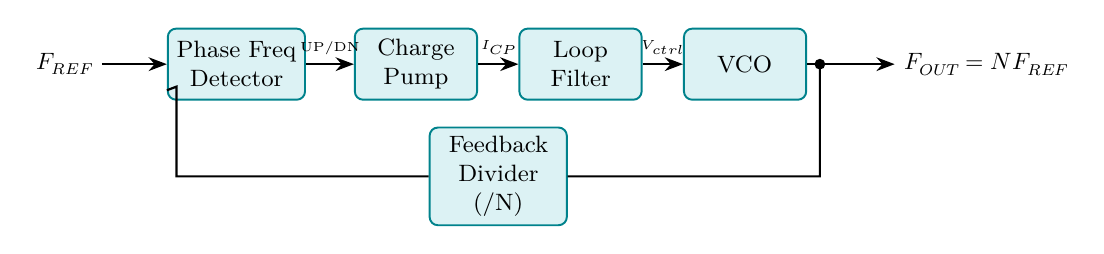
\begin{tikzpicture}[scale=0.95, transform shape]
  % PFD
  \node[block, text width=1.6cm] (pfd) at (0, 0) {Phase Freq\\Detector};
  
  % CP
  \node[block, text width=1.4cm] (cp) at (2.4, 0) {Charge\\Pump};
  
  % LF
  \node[block, text width=1.4cm] (lf) at (4.6, 0) {Loop\\Filter};
  
  % VCO
  \node[block, text width=1.4cm] (vco) at (6.8, 0) {VCO};
  
  % Divider
  \node[block, text width=1.6cm] (div) at (3.5, -1.5) {Feedback\\Divider (/N)};

  % Paths
  \draw[-Stealth, thick] (-1.8, 0) node[left, font=\small] {$F_{REF}$} -- (pfd);
  \draw[-Stealth, thick] (pfd) -- (cp) node[midway, above, font=\tiny] {UP/DN};
  \draw[-Stealth, thick] (cp) -- (lf) node[midway, above, font=\tiny] {$I_{CP}$};
  \draw[-Stealth, thick] (lf) -- (vco) node[midway, above, font=\tiny] {$V_{ctrl}$};
  \draw[-Stealth, thick] (vco) -- (8.8, 0) node[right, font=\small] {$F_{OUT} = N F_{REF}$};
  
  % Feedback path
  \draw[thick] (7.8, 0) to[short, *-] (7.8, -1.5) -- (div);
  \draw[thick] (div) -| (-0.8, -0.8) -- (-0.8, -0.3) -- (pfd);
\end{tikzpicture}
\end{tcolorbox}

\textbf{Working of Each Block:}
\begin{enumerate}[label=\textbf{\arabic*.}, leftmargin=*, itemsep=3pt]
  \item \textbf{Phase Frequency Detector (PFD):} Compares the reference clock $F_{REF}$ with the feedback clock $F_{FB}$. It generates digital pulses (UP and DN) whose widths are proportional to the phase and frequency difference between the inputs.
  \item \textbf{Charge Pump (CP):} Converts the digital UP/DN control pulses into a proportional current charge injection:
  \[
  I_{avg} = I_{CP} \frac{\Delta \Phi}{2\pi}
  \]
  \item \textbf{Loop Filter (LF):} A passive low-pass filter (usually a resistor $R$ in series with a capacitor $C_1$, in parallel with a smaller capacitor $C_2$). It integrates the CP current to generate a smooth analog tuning voltage $V_{ctrl}$.
  \item \textbf{Voltage Controlled Oscillator (VCO):} A circuit whose output frequency is controlled by $V_{ctrl}$. The output frequency is:
  \[
  \omega_{out} = \omega_{fr} + K_{VCO} V_{ctrl}
  \]
  where $\omega_{fr}$ is the free-running frequency and $K_{VCO}$ is the VCO gain (rad/s/V).
  \item \textbf{Feedback Divider (/N):} Divides the high output frequency down to the reference frequency, allowing the loop to lock at $F_{OUT} = N F_{REF}$.
\end{enumerate}

\subsection{Mathematical Loop Dynamics (Type-II CP-PLL)}
A Type-II PLL has two integrators in the loop: the VCO (which integrates frequency to phase: $\Phi_{out} = \int \omega_{out} dt \Rightarrow H_{VCO}(s) = K_{VCO}/s$) and the loop filter (which contains an integrating capacitor).

\textbf{Transfer Functions of Components:}
\begin{itemize}[leftmargin=*, itemsep=2.5pt]
  \item PFD/CP Gain: $K_d = \frac{I_{CP}}{2\pi}$ (A/rad).
  \item Loop Filter Impedance: $Z_{LF}(s) = R + \frac{1}{s C_1} = \frac{1 + s R C_1}{s C_1}$ (ignoring the small parallel capacitor $C_2$).
  \item VCO Transfer Function: $H_{VCO}(s) = \frac{K_{VCO}}{s}$.
\end{itemize}

\textbf{Open-Loop Gain $A(s)$:}
\[
A(s) = K_d \cdot Z_{LF}(s) \cdot \frac{H_{VCO}(s)}{N} = \left(\frac{I_{CP}}{2\pi}\right) \left(\frac{1 + s R C_1}{s C_1}\right) \left(\frac{K_{VCO}}{s}\right) \frac{1}{N}
\]
\[
A(s) = \frac{I_{CP} K_{VCO} (1 + s R C_1)}{2\pi N C_1 s^2}
\]

\textbf{Closed-Loop Transfer Function $H_{cl}(s) = \frac{\Phi_{out}(s)}{\Phi_{in}(s)}$:}
\[
H_{cl}(s) = \frac{N \cdot A(s)}{1 + A(s)} = \frac{\frac{I_{CP} K_{VCO} R}{2\pi} s + \frac{I_{CP} K_{VCO}}{2\pi C_1}}{s^2 + \frac{I_{CP} K_{VCO} R}{2\pi N} s + \frac{I_{CP} K_{VCO}}{2\pi N C_1}}
\]

Comparing this with the standard second-order system denominator $s^2 + 2\zeta\omega_n s + \omega_n^2$:
\begin{tcolorbox}[formulabox, title={\textbf{Type-II CP-PLL Dynamics}}]
\textbf{Natural Frequency ($\omega_n$):}
\[
\omega_n = \sqrt{\frac{I_{CP} K_{VCO}}{2\pi N C_1}}
\]
\textbf{Damping Factor ($\zeta$):}
\[
\zeta = \frac{R C_1}{2} \omega_n = \frac{R}{2} \sqrt{\frac{I_{CP} K_{VCO} C_1}{2\pi N}}
\]
\end{tcolorbox}
The resistor $R$ is critical; it introduces a zero in the open-loop transfer function, stabilizing the second-order feedback loop by providing adequate phase margin (damping).

\subsection{VCO Design: Ring Oscillator vs.~LC-Tank}
The VCO is the most noise-sensitive block in the PLL. Two dominant topologies are used:

\begin{tcolorbox}[tikzbox, title={3-Stage Ring Oscillator and LC-Tank Resonator Diagrams}]
\centering
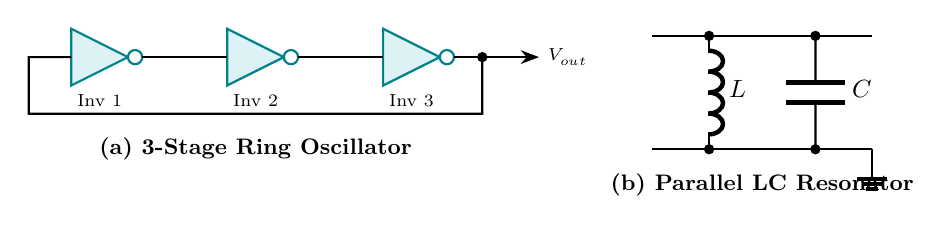
\begin{tikzpicture}[scale=0.9, transform shape]
  % Ring Oscillator (Left)
  \begin{scope}[xshift=0cm]
    % 3 inverters
    \foreach \i in {1, 2, 3} {
      \pgfmathsetmacro{\x}{(\i-1)*2.2}
      % Triangle
      \draw[thick, fill=hdrteal, draw=myteal] (\x, 0.4) -- (\x, -0.4) -- (\x+0.8, 0) -- cycle;
      % Circle
      \draw[thick, draw=myteal, fill=white] (\x+0.9, 0) circle (0.1);
      \node[below, font=\scriptsize] at (\x+0.4, -0.4) {Inv \i};
    }
    
    % Connections between inverters
    \draw[thick] (0.9+0.1, 0) -- (2.2, 0);
    \draw[thick] (2.2+0.9+0.1, 0) -- (4.4, 0);
    \draw[thick] (4.4+0.9+0.1, 0) -- (6.0, 0);
    
    % Feedback loop
    \draw[thick] (5.8, 0) to[short, *-] (5.8, -0.8) -- (-0.6, -0.8) -- (-0.6, 0) -- (0, 0);
    \draw[-Stealth, thick] (6.0, 0) -- (6.6, 0) node[right, font=\scriptsize] {$V_{out}$};
    
    \node[font=\small\bfseries] at (2.6, -1.3) {(a) 3-Stage Ring Oscillator};
  \end{scope}

  % LC Resonator (Right)
  \begin{scope}[xshift=9.0cm, yshift=0.3cm]
    % Parallel L and C
    \draw[thick] (0, 0) to[L, l=$L$, *-*] (0, -1.6);
    \draw[thick] (1.5, 0) to[C, l=$C$, *-*] (1.5, -1.6);
    
    % Top and bottom rails
    \draw[thick] (-0.8, 0) -- (2.3, 0);
    \draw[thick] (-0.8, -1.6) -- (2.3, -1.6) node[ground] {};
    
    \node[font=\small\bfseries] at (0.75, -2.1) {(b) Parallel LC Resonator};
  \end{scope}
\end{tikzpicture}
\end{tcolorbox}

\begin{tcolorbox}[tikzbox, title={Ring Oscillator vs.~LC-Tank VCO Comparison}]
\centering
\par\noindent
\renewcommand{\arraystretch}{1.3}
\begin{tabularx}{\linewidth}{|B{3.0cm}|Y|Y|}
\hline
\textbf{Property} & \textbf{Ring Oscillator VCO} & \textbf{LC-Tank VCO} \\ \hline
\textbf{Structure} & $N$ cascaded inverter/delay stages in a ring & Parallel LC resonator with varactor for tuning \\ \hline
\textbf{Phase Noise} & Poor ($-90$ to $-100\,$dBc/Hz at 1\,MHz) & Excellent ($-120$ to $-145\,$dBc/Hz at 1\,MHz) \\ \hline
\textbf{Tuning Range} & Very wide ($>2\times$) & Narrow ($\sim 10$--$20\%$) \\ \hline
\textbf{Silicon Area} & Very compact (inverters only) & Large (on-chip inductor is bulky) \\ \hline
\textbf{Frequency} & DC to $>10\,$GHz (digital CMOS) & $500\,$MHz to $>60\,$GHz \\ \hline
\textbf{Applications} & Digital CDR, on-chip clocking & RF synthesizers, wireless transceivers \\ \hline
\end{tabularx}
\end{tcolorbox}

% ===============================================================================
\section{Delay-Locked Loop (DLL) Architecture \& Working}
% ===============================================================================

\begin{tcolorbox}[defbox, title={\textbf{Delay-Locked Loop (DLL) Concept}}]
A \textbf{Delay-Locked Loop (DLL)} is a feedback system that aligns the phase of an output clock with an input clock by controlling the delay of a Voltage-Controlled Delay Line (VCDL). Unlike a PLL, a DLL does not use an oscillator (VCO); it only shifts the phase of an existing clock.
\end{tcolorbox}

\subsection{Block Components and Signal Flow}
A DLL consists of a Phase Detector (PD), a Charge Pump (CP), a Loop Filter (LF), and a Voltage-Controlled Delay Line (VCDL).

\begin{tcolorbox}[tikzbox, title={Block Diagram of a Delay-Locked Loop}]
\centering
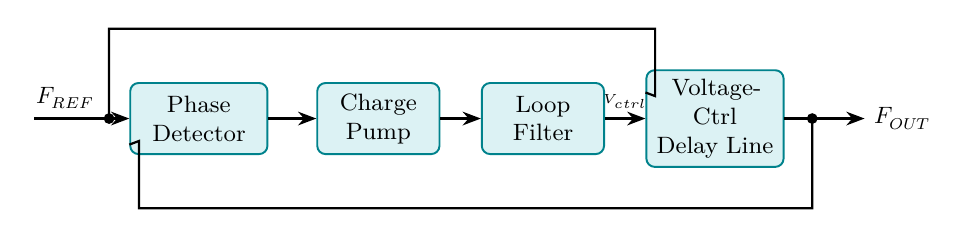
\begin{tikzpicture}[scale=0.95, transform shape]
  % PD
  \node[block, text width=1.6cm] (pd) at (0, 0) {Phase\\Detector};
  
  % CP
  \node[block, text width=1.4cm] (cp) at (2.4, 0) {Charge\\Pump};
  
  % LF
  \node[block, text width=1.4cm] (lf) at (4.6, 0) {Loop\\Filter};
  
  % VCDL
  \node[block, text width=1.6cm] (vcdl) at (6.9, 0) {Voltage-Ctrl\\Delay Line};

  % Paths
  \draw[-Stealth, thick] (-2.2, 0) -- (pd);
  \node[above, font=\small] at (-1.8, 0) {$F_{REF}$};
  \draw[thick] (-1.2, 0) to[short, *-] (-1.2, 1.2) -- (6.1, 1.2) -- (6.1, 0.3) -- (vcdl);
  
  \draw[-Stealth, thick] (pd) -- (cp);
  \draw[-Stealth, thick] (cp) -- (lf);
  \draw[-Stealth, thick] (lf) -- (vcdl) node[midway, above, font=\tiny] {$V_{ctrl}$};
  
  \draw[-Stealth, thick] (vcdl) -- (8.9, 0) node[right, font=\small] {$F_{OUT}$};
  
  % Feedback path
  \draw[thick] (8.2, 0) to[short, *-] (8.2, -1.2) -| (-0.8, -0.6) -- (-0.8, -0.3) -- (pd);
\end{tikzpicture}
\end{tcolorbox}

\subsection{PLL vs. DLL Stability \& Jitter Comparison}

\begin{tcolorbox}[tikzbox, title={Comparison of PLL and DLL Architectures}]
\centering
\par\noindent
\begin{tabularx}{\linewidth}{|B{3.2cm}|Y|Y|}
\hline
\textbf{Parameter} & \textbf{Phase-Locked Loop (PLL)} & \textbf{Delay-Locked Loop (DLL)} \\ \hline
\textbf{Core Component} & VCO (Voltage Controlled Oscillator) & VCDL (Voltage Controlled Delay Line) \\ \hline
\textbf{System Order} & Type-II, 2nd-order or higher (requires series $R$ to stabilize) & Type-I, 1st-order system (unconditionally stable) \\ \hline
\textbf{Jitter Behavior} & \textbf{Jitter Accumulation:} Noise recirculates in the VCO tank/ring, accumulating over cycles & \textbf{No Jitter Accumulation:} Jitter is reset at the end of the delay line every cycle \\ \hline
\textbf{Frequency Synthesis} & Supports frequency multiplication ($F_{OUT} = N F_{REF}$) & Cannot multiply frequency directly; only shifts phase \\ \hline
\textbf{Lock Range} & Limited by VCO tuning range and loop dynamics & Limited by VCDL delay range; prone to harmonic locking \\ \hline
\end{tabularx}
\end{tcolorbox}

\begin{itemize}[leftmargin=*, itemsep=2.5pt]
  \item \textbf{Stability Analysis:} The VCDL is a simple delay stage. Unlike a VCO, it does not integrate frequency to phase (it has no $1/s$ phase term). The DLL closed-loop system is first-order, meaning it is unconditionally stable and the loop filter requires only a single capacitor (no resistor $R$ is needed).
  \item \textbf{Jitter Analysis:} In a VCO, if a clock edge is delayed due to noise, the subsequent edges remain shifted because the phase error accumulates over time. In a VCDL, the input clock is a clean external clock. Any noise-induced delay inside the VCDL affects only the current cycle; the next cycle starts with a fresh, clean reference edge.
\end{itemize}

% ===============================================================================
\section{Digital PLLs \& Frequency Synthesizers}
% ===============================================================================

\subsection{Digital PLL (DPLL) and All-Digital PLL (ADPLL)}
Modern SOCs implement ADPLLs to avoid bulky analog capacitors and process scaling issues:
\begin{itemize}[leftmargin=*, itemsep=2pt]
  \item \textbf{TDC:} A Time-to-Digital Converter replaces the PFD, converting phase differences directly into digital words.
  \item \textbf{Digital Loop Filter (DLF):} Replaces the analog loop filter, saving silicon area and allowing programmable tuning coefficients.
  \item \textbf{DCO:} A Digitally Controlled Oscillator replaces the VCO, using capacitor DAC banks to control oscillation frequency.
\end{itemize}

\subsection{Frequency Synthesizers}
Synthesizers generate multiple frequencies from a single reference:
\begin{itemize}[leftmargin=*, itemsep=2.5pt]
  \item \textbf{Integer-N Synthesizer:} Output frequency is $F_{OUT} = N F_{REF}$. The step size is limited to $F_{REF}$.
  \item \textbf{Fractional-N Synthesizer:} The feedback divider toggles between $N$ and $N+1$ using a Delta-Sigma modulator. This allows the average division ratio to be fractional, providing fine frequency steps with a high reference frequency (reducing loop division noise).
\end{itemize}

% ===============================================================================
% QUICK REVISION PAGE
% ===============================================================================
\newpage
\begin{center}
  {\large\bfseries\color{myred} Quick Revision --- Module 5}\\[3pt]
  {\small\color{mydark} PLLs \& DLLs $|$ PE-EC802A}
\end{center}
\noindent{\color{myred}\rule{\linewidth}{1.2pt}}
\vspace{4pt}

\begin{tcolorbox}[formulabox, title={\textbf{Key Formulas at a Glance}}]
\renewcommand{\arraystretch}{1.35}
\begin{tabularx}{\linewidth}{B{5.0cm} X}
VCO Output Frequency & $\omega_{out} = \omega_{fr} + K_{VCO} V_{ctrl}$ \\[4pt]
PFD/CP Gain & $K_d = \frac{I_{CP}}{2\pi}$ \\[4pt]
VCO Phase integration & $H_{VCO}(s) = \frac{K_{VCO}}{s}$ \\[4pt]
Loop Natural Frequency & $\omega_n = \sqrt{\frac{I_{CP} K_{VCO}}{2\pi N C_1}}$ \\[4pt]
Loop Damping Factor & $\zeta = \frac{R}{2} \sqrt{\frac{I_{CP} K_{VCO} C_1}{2\pi N}}$ \\[4pt]
Integer-N output & $F_{OUT} = N F_{REF}$ \\
\end{tabularx}
\end{tcolorbox}

\begin{tcolorbox}[defbox, title={\textbf{One-Line Definitions}}]
\begin{itemize}[leftmargin=*, itemsep=2pt, topsep=0pt]
  \item \textbf{VCO:} An oscillator whose output frequency is a linear function of its input control voltage.
  \item \textbf{PFD:} A phase-detector block that detects both phase and frequency differences, preventing false lock states.
  \item \textbf{Loop Filter:} A low-pass filter that filters out the high-frequency charge-pump ripple to generate a smooth control voltage.
  \item \textbf{Damping Factor:} A parameter that determines the stability and transient settling time of the PLL loop.
  \item \textbf{VCDL:} A line of buffer stages whose propagation delay is controlled by an input voltage.
  \item \textbf{ADPLL:} A phase-locked loop consisting entirely of digital components (TDC, Digital Filter, DCO).
  \item \textbf{Fractional-N Synthesizer:} A frequency synthesizer that achieves fractional division ratios by dynamically switching divider counts.
\end{itemize}
\end{tcolorbox}

\begin{tcolorbox}[tikzbox, title={\textbf{PLL vs.~DLL Architecture Comparison}}]
\centering
\par\noindent
\renewcommand{\arraystretch}{1.3}
\begin{tabularx}{\linewidth}{|B{3.0cm}|Y|Y|}
\hline
\textbf{Property} & \textbf{Phase-Locked Loop (PLL)} & \textbf{Delay-Locked Loop (DLL)} \\ \hline
\textbf{Core block} & VCO (integrates freq.~to phase) & VCDL (shifts phase, no integration) \\ \hline
\textbf{System order} & 2nd-order (Type-II), needs $R$ to stabilize & 1st-order, unconditionally stable \\ \hline
\textbf{Jitter} & Accumulates (VCO noise recirculates) & Non-accumulating (reset each cycle) \\ \hline
\textbf{Freq.~synthesis} & Yes: $F_{out} = N F_{ref}$ & No (phase shift only) \\ \hline
\textbf{Lock range} & Limited by VCO tuning range & Limited by VCDL delay range \\ \hline
\textbf{Application} & Frequency synthesis, clocking & Deskew, phase alignment \\ \hline
\end{tabularx}
\end{tcolorbox}

\begin{tcolorbox}[exambox, title={\textbf{Frequently Asked / Viva Questions}}]
\begin{enumerate}[topsep=0pt, label=\textbf{Q\arabic*.}, itemsep=5pt]
  \item \Q{What are the main blocks of a charge-pump PLL?}
    The five main blocks are the Phase Frequency Detector (PFD), Charge Pump (CP), Loop Filter (LF), Voltage-Controlled Oscillator (VCO), and the Feedback Divider (/N).
  \item \Q{Why is a resistor needed in series with the capacitor in a PLL loop filter?}
    The VCO acts as an integrator ($1/s$). If the loop filter is a simple capacitor, it acts as a second integrator ($1/s$). This creates two poles at the origin, making the system unstable (phase margin is $0^\circ$). The resistor introduces a zero ($1+sRC$) that restores stability.
  \item \Q{Compare PLL and DLL stability.}
    A DLL is a first-order system because the VCDL only shifts phase and does not integrate frequency to phase. Therefore, it is unconditionally stable. A PLL is a second-order (or higher) system due to the VCO phase integration and loop filter, requiring careful stabilization.
  \item \Q{Explain the difference in jitter behavior between a PLL and a DLL.}
    In a PLL, phase errors recirculate through the VCO feedback loop, leading to jitter accumulation over time. In a DLL, the input reference clock is clean, and the jitter is reset at the end of the VCDL line every clock cycle, preventing jitter accumulation.
  \item \Q{What is a Phase Frequency Detector (PFD), and what is its advantage over a simple XOR Phase Detector?}
    An XOR PD only detects phase difference and can lock to harmonics or fail to lock if frequencies are different. A PFD detects both phase and frequency differences, ensuring the loop always locks to the correct frequency.
  \item \Q{What is frequency multiplication in a PLL, and how is it achieved?}
    Frequency multiplication allows generating a high frequency output $F_{OUT} = N F_{REF}$ from a low frequency reference. It is achieved by placing a divide-by-$N$ counter in the feedback path, forcing the VCO to run $N$ times faster to lock.
  \item \Q{What is a Digitally Controlled Oscillator (DCO) and where is it used?}
    A DCO is an oscillator whose output frequency is controlled by digital inputs (typically selecting capacitors in a varactor DAC array). It is a core block in All-Digital PLLs (ADPLLs).
  \item \Q{Explain the working of a fractional-N synthesizer.}
    A fractional-N synthesizer achieves a fractional division ratio (e.g. $N.25$) by dynamically toggling the feedback divider value between $N$ and $N+1$ (e.g., dividing by $N$ for 75\% of the time and $N+1$ for 25\% of the time). A Delta-Sigma modulator is used to shape the divider switching noise.
  \item \Q{What is the function of the charge pump in a PLL?}
    It converts the digital UP and DN pulses from the PFD into analog current pulses, injecting or extracting charge from the loop filter to adjust the VCO control voltage.
  \item \Q{What is a Time-to-Digital Converter (TDC)?}
    A TDC is a digital circuit that measures the time interval between two clock transitions and outputs it as a digital word. It replaces the analog PFD/CP in digital PLLs.
\end{enumerate}
\end{tcolorbox}


\end{document}
